\documentclass[11pt,a4paper]{book}
\usepackage[margin=2in]{geometry}
\usepackage[italian]{babel}
\usepackage[T1]{fontenc}
\usepackage[utf8]{inputenc}
\usepackage{graphicx}
\usepackage{imakeidx}
\usepackage{amsmath}
\usepackage{color}


\usepackage[hyperfootnotes=false, colorlinks=true, linkcolor=black]{hyperref}
\usepackage[style=numeric-comp,useprefix,hyperref,backend=bibtex]{biblatex}
\usepackage{listings}  % Serve per evidenziare i blocchi di codice
\usepackage{pxfonts} % permette di avere caratteri in lstlisting con formattazione

\setlength{\parskip}{1em} % cambia l'interlinea prima di un nuovo capoverso

% Colori per lstlisting
\definecolor{pblue}{rgb}{0.13,0.13,1}
\definecolor{pgreen}{rgb}{0,0.5,0}
\definecolor{pred}{rgb}{0.9,0,0}
\definecolor{pgrey}{rgb}{0.46,0.45,0.48}
\definecolor{maroon}{rgb}{0.5,0,0}
\definecolor{plightgrey}{rgb}{0.8,0.8,0.8} 


\usepackage{xcolor} % Necessario per definire i colori
\hypersetup{
  colorlinks=true,
  linkcolor=green!70!black,
  urlcolor=green!70!black
} % Setup colore link


\lstset{ % Riduce la larghezza della tabulazione per lstlisting
  tabsize=2,
  backgroundcolor=\color{plightgrey},
  breaklines=true,
  postbreak=\mbox{\textcolor{red}{$\hookrightarrow$}\space},
  columns=fullflexible,
  frame=single,
}


\lstset{
  language=XML,
  basicstyle=\ttfamily,
  morestring=[s]{"}{"},
  morecomment=[s]{?}{?},
  morecomment=[s]{!--}{--},
  commentstyle=\color{white},
  moredelim=[s][\color{black}]{>}{<},
  moredelim=[s][\color{red}]{\ }{=},
  stringstyle=\color{blue},
  identifierstyle=\color{maroon}
}
% Crea un set di impostazioni per Java in lstlisting
\lstset{language=Java,
  showspaces=false,
  showtabs=false,
  breaklines=true,
  showstringspaces=false,
  breakatwhitespace=true,
  commentstyle=\color{white},
  keywordstyle=\color{pblue},
  stringstyle=\color{pred},
  basicstyle=\ttfamily,
  moredelim=[is][\textcolor{pgrey}]{\%\%}{\%\%}
}

% Crea un set di impostazioni per C++ in lstlisting
\lstset{language=C++,
                basicstyle=\ttfamily,
                keywordstyle=\color{blue}\ttfamily,
                stringstyle=\color{red}\ttfamily,
                commentstyle=\color{white}\ttfamily,
                morecomment=[l][\color{magenta}]{\#}
}

\begin{document}
\title{Testing - teoria e pratica in Java}
\author{Jacopo De Angelis}
\maketitle

\pagebreak
\tableofcontents
\pagebreak

\chapter{Software quality}
È il livello di conformità ai requisiti impliciti ed espliciti.

\paragraph{Definizione}
Il grado con il quale il sistema, componente, o processo incontra sia i requisiti che le aspettative dell'utente.

\paragraph{Spiegazione}
\begin{itemize}
	\item \textbf{Espliciti}: Definiti e documentati
	\item \textbf{Impliciti}: Non chiaramente definiti ma comunque consigliati
	\item \textbf{Requisiti}: Legati al business, al prodotto o al software
	\item \textbf{Aspettative}: Principalmente le aspettative dell'utente
\end{itemize}

\section{Dimensione della software quality}
Ci sono svariate dimensioni utilizzate, queste sono solo alcune. La loro importanza è soggettiva e dipende dalla situazione.

\begin{itemize}
	\item \textbf{Accessibilità}: Livello al quale il software può essere usato in maniera confortevole dalle persone, comprese le persone che hanno handicap di utilizzo
	\item \textbf{Compatibilità}: L'adeguatezza del software usato in diversi ambienti come differenti dispositivi, sistemi operativi e browser
	\item \textbf{Concorrenza}: L'abilità del software di soddisfare richieste multiple contemporaneamente
	\item \textbf{Efficienza}: L'abilità del software di lavorare bene o raggiungere il risultato senza sprecare energie, risorse, tempo o denaro
	\item \textbf{Funzionalità}: L'abilità del software di eseguire le funzioni come richiesto
	\item \textbf{Installabilità}: L'abilità del software di essere installato in vari ambienti
	\item \textbf{Localizzazione}: L'abilità del software di essere utilizzato in lingue differenti, time zones, ecc.
	\item \textbf{Manutenibilità}: La semplicità con la quale il software può essere modificato
	\item \textbf{Performance}: La velocità con la quale il software lavora sotto certi carichi
	\item \textbf{Portabilità}: L'abilità del software di essere trasferito facilmente da una piattafroma ad un'altra
	\item \textbf{Affidabilità}: L'abiità del softwaredi eseguire le funzioni richieste sotto certe condizioni per un determinato periodo di tempo senza errori
	\item \textbf{Scalabilità}: La misura nella quale il software può aumentare o decrementare le performance in risposta alle domande di lavoro del software
	\item \textbf{Sicurezza}: La sicurezza del software contro accessi non autorizzati, invasione della privacy, furto, perdita di dati, ecc.
	\item \textbf{Testabilità}: L'abilità del software di essere testato
	\item \textbf{Usablità}: Quanto il software è semplice da utilizzare
\end{itemize}

\section{Software Quality Assurance (SQA)}
È un insieme di attività per assicurare la qualità nel processo di creazione del software che risulta, o almeno offre un certo grado di sicurezza, in una qualità superiore del software.

La SQA accompagna tutto il ciclo di vita dello sviluppo software e il suo obiettivo è di assicurare che lo sviluppo e il processo di manutenzione siano continuamente migliorati per produrre prodotti che incontrano lo specifiche.

Una volt terminato il processo di sviluppo, QA ha lo scopo di trovare le debolezze nel processo e correggerle per continuare a migliorarlo.

\section{Software Quality Control}
È l'insieme di attività per assicurare la qualità nel processo di controllo qualità del software. La SQC è limitata alla fase di Review/Testing nel ciclo di vita del software e l'obiettivo è quello di assicurare che il prodotto incontri i requisiti.

\section{Verifica vs validazione}
Sono spesso confusi.
\begin{table}[]
\begin{tabular}{|c|l|l|}
\hline
\textbf{Criterio}                                                            & \multicolumn{1}{c|}{\textbf{Verifica}}                                                                                                                                                                                         & \multicolumn{1}{c|}{\textbf{Validazione}}                                                                                                                                                                                                                                     \\ \hline
\textbf{Definizione}                                                         & \begin{tabular}[c]{@{}l@{}}Il processo di valutazione\\ del prodotto durante lo\\ sviluppo per determinare\\ se incontra i requisiti \\ richiesti in quella fase\end{tabular}                                                  & \begin{tabular}[c]{@{}l@{}}Il processo di valutazione\\ del software durante o\\ alla fine dello sviluppo \\ per determinare se\\ rispetta i requisiti del\\ business\end{tabular}                                                                                            \\ \hline
\textbf{Obiettivo}                                                           & \begin{tabular}[c]{@{}l@{}}Assicurarsi che il prodotto\\ sia creato in accordo con\\ le richieste e le specifiche\\ di desgin. In altre parole, \\ per assicurarsi che il lavoro\\ incontri i requisiti specifici\end{tabular} & \begin{tabular}[c]{@{}l@{}}Assicurarsi che il prodotto \\ incontri le necessità dell'\\ utente e che le specifiche\\ siano corrette dal principio.\\ In altre parole, dimostrare\\ che il prodotto soddisfa il\\ suo caso d'uso quanto \\ messo nel suo ambiente\end{tabular} \\ \hline
\textbf{Domanda}                                                             & \begin{tabular}[c]{@{}l@{}}Stiamo costruendo qualcosa\\ in maniera corretta?\end{tabular}                                                                                                                                      & \begin{tabular}[c]{@{}l@{}}Stiamo costruendo il \\ prodotto corretto?\end{tabular}                                                                                                                                                                                            \\ \hline
\textbf{\begin{tabular}[c]{@{}c@{}}Oggetti della\\ valutazione\end{tabular}} & \begin{tabular}[c]{@{}l@{}}Piani, specifiche, design, \\ codice, casi di test\end{tabular}                                                                                                                                     & Il software                                                                                                                                                                                                                                                                   \\ \hline
\textbf{Attività}                                                            & Review, percorsi, ispezioni                                                                                                                                                                                                    & Testing                                                                                                                                                                                                                                                                       \\ \hline
\end{tabular}
\end{table}

\section{Software Development Life Cycle (SDLC)}
Definisce le fasi della costruzione del software. Il ciclo di vita varia tra i vari modelli e ci sono vari tipi di modelli:
\begin{itemize}
	\item Waterfall
	\item Spirale
	\item Iterativo ed incrementale
	\item Agile
\end{itemize}

\section{Software Testing Life Cycle (STLC)}
Definisce i vari stati della vita di testing del software. Non ci sono standard condivisi. L'unica cosa certa è che generalmente condivide questi passi:
\begin{figure}[h!]
	\begin{center}
		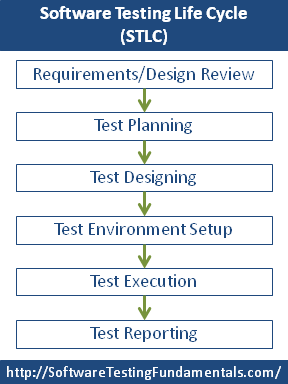
\includegraphics[scale=0.6]{img/004.png}
		\caption{STLC}
		\label{fig: 004}
	\end{center}
\end{figure}

\chapter{Cos'è il test driven development?}
In informatica, nello sviluppo software, il test-driven development (abbreviato in TDD) è un modello di sviluppo del software che prevede che la stesura dei test automatici avvenga prima di quella del software che deve essere sottoposto a test, e che lo sviluppo del software applicativo sia orientato esclusivamente all'obiettivo di passare i test automatici precedentemente predisposti.

Più in dettaglio, il TDD prevede la ripetizione di un breve ciclo di sviluppo in tre fasi:
\begin{enumerate}
	\item \textbf{Fase rossa}: il programmatore scrive un test automatico per la nuova funzione da sviluppare, che deve fallire in quanto la funzione non è stata ancora realizzata.
	\item \textbf{Fase verde}: il programmatore sviluppa la quantità minima di codice necessaria per passare il test.
	\item \textbf{Fase grigia, refactoring}: il programmatore esegue il refactoring del codice per adeguarlo a determinati standard di qualità.
\end{enumerate}

Il TDD consta di quattro fasi di testing:
\begin{figure}[h!]
	\begin{center}
		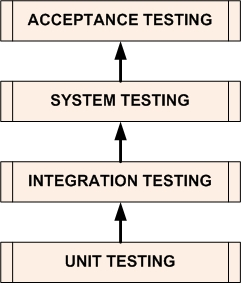
\includegraphics[scale=0.6]{img/002.jpg}
		\caption{Livelli di testing}
		\label{fig: 002}
	\end{center}
\end{figure}
\begin{itemize}
	\item \textbf{Unit testing}: A questo livello le singole componenti vengono testate. Lo scopo è quello di validare ogni unità
	\item \textbf{Integraion testing}: A questo livello le singole unità sono combinate e testate in gruppo. Lo scopo è quello di esporre i difetti di integrazione tra le unità
	\item \textbf{System testing}: A questo livello l'intero sistema è testato. Lo scopo è quello di valutare il rispetto di requisiti specifici	
	\item \textbf{Acceptance testing}: A questo livello il sistema è testato per la sua accettazione. Lo scopo è quello di valutare il rispetto dei criteri di accettazione del sistema	 
\end{itemize}

In più c'è il regression testing che accomuna tutte queste categorie, ovvero è un livello che controlla che il nuovo codice non abbia avuto effetti negativi sul codice già testato.

\section{Cicli TDD}
La definizione originale è stata data da Kent Back.
\begin{figure}[h!]
	\begin{center}
		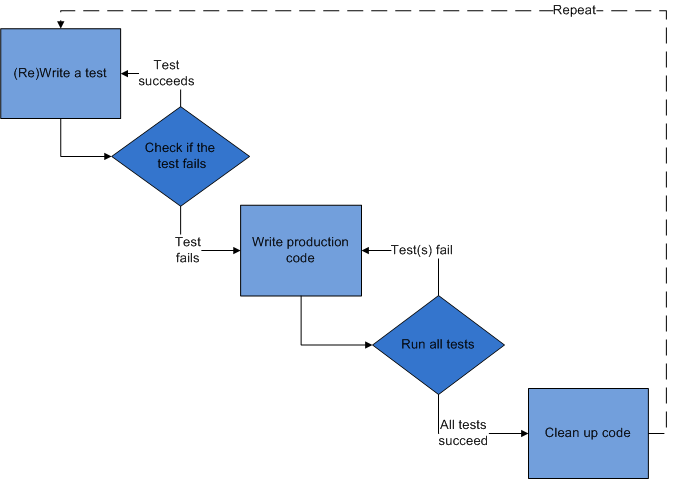
\includegraphics[scale=0.6]{img/001.png}
		\caption{Rappresentazione del TDD}
		\label{fig: 001}
	\end{center}
\end{figure}

\subsection{Fase rossa}
Nel TDD, lo sviluppo di una nuova funzionalità \textbf{comincia} sempre \textbf{con la stesura di un test automatico volto a validare quella funzionalità}, ovvero verificare se il software la esibisce. Poiché l'implementazione non esiste ancora, la stesura del test è un'attività creativa, in quanto il programmatore deve stabilire in quale forma la funzionalità verrà esibita dal software e comprenderne e definirne i dettagli. 

Perché il test sia completo, deve essere eseguibile e, quando viene eseguito, produrre un esito negativo. In molti contesti, questo implica che debba essere realizzato uno "stub" minimale del codice da testare, anche solo definire l'intestazione dei metodi, necessario per garantire la compilabilità e l'eseguibilità del test. 

Una volta che il nuovo test è completo e può essere eseguito, dovrebbe fallire. \textbf{La fase rossa si conclude quando c'è un nuovo test che può essere eseguito e fallisce.}

\subsection{Fase verde}
Nella fase successiva, \textbf{il programmatore deve scrivere la quantità minima di codice necessaria per passare il test che fallisce.} Non è richiesto che il codice scritto sia di buona qualità, elegante, o generale; \textbf{l'unico obiettivo esplicito è che funzioni, ovvero passi il test.} 

In effetti, è esplicitamente vietato dalla pratica del TDD lo sviluppo di parti di codice non strettamente finalizzate al superamento del test che fallisce. Quando il codice è pronto, il programmatore lancia nuovamente tutti i test disponibili sul software modificato (non solo quello che precedentemente falliva). In questo modo, il programmatore ha modo di rendersi conto immediatamente se la nuova implementazione ha causato fallimenti di test preesistenti, ovvero ha causato regression nel codice. 

\textbf{La fase verde termina quando tutti i test sono "verdi" (ovvero vengono passati con successo)}.

\subsection{Fase grigia, refactoring}
Quando il software passa tutti i test, \textbf{il programmatore dedica una certa quantità di tempo a farne refactoring, ovvero a migliorarne la struttura attraverso un procedimento basato su piccole modifiche controllate volte a eliminare o ridurre difetti oggettivamente riconoscibili nella struttura interna del codice}. 

Esempi tipici di azioni di refactoring includono la scelta di identificatori più espressivi, eliminazione di codice duplicato, semplificazione e razionalizzazione dell'architettura del sorgente (p.es. in termini della sua organizzazione in classi), e così via. 

La letteratura sul TDD fornisce numerose linee guida sia specifiche che generali sul modo corretto di fare refactoring. In ogni caso, l'obiettivo del refactoring non è quello di ottenere del codice "perfetto", ma solo di migliorarne la struttura, secondo la cosiddetta "regola dei Boy Scout": "lascia l'area dove ti sei accampato più pulita di come l'hai trovata". 

\textbf{Dopo ciascuna azione di refactoring, i test automatici vengono nuovamente eseguiti per accertarsi che le modifiche eseguite non abbiano introdotto errori}.
\textbf{Il principio fondamentale del TDD è che lo sviluppo vero e proprio deve avvenire solo allo scopo di passare un test automatico che fallisce.} In particolare, questo vincolo è inteso a \textbf{impedire che il programmatore sviluppi funzionalità non esplicitamente richieste, e che il programmatore introduca complessità eccessiva in un progetto}, per esempio perché prevede la necessità di generalizzare l'implementazione in un futuro più o meno prossimo. 

In questo senso il TDD è in stretta relazione con numerosi principi della programmazione agile e dell'extreme programming, come il principio \textbf{KISS (Keep It Simple, Stupid)}, il principio \textbf{YAGNI (You aren't gonna need it)}, e il mandato agile di massimizzare la quantità di lavoro non fatto.

\textbf{I cicli TDD sono intesi come cicli di breve durata, al termine di ciascuno dei quali il programmatore ha realizzato un piccolo incremento di prodotto} (con i relativi test automatici), un altro concetto tipico delle metodologie agili.\textbf{ L'applicazione reiterata del refactoring al termine di ogni ciclo ha lo scopo di creare codice di alta qualità e buone architetture in modo incrementale}, tenendo però separati l'obiettivo di costruire software funzionante (fase verde) e quello di scrivere "buon codice" (fase grigia). La breve durata dei cicli TDD tende anche a favorire lo sviluppo di componenti di piccole dimensioni e ridotta complessità.

L'applicazione del TDD porta in generale allo sviluppo di un numero maggiore di test, e a una maggiore copertura di test del software prodotto, rispetto alla pratica tradizionale di sviluppare i test dopo l'implementazione. In parte, questo è dovuto al fatto che in contesti non TDD il management tende a spingere i programmatori a passare all'implementazione di nuove funzionalità a scapito del completamento dei test. \textbf{I programmatori che usano il TDD su progetti nuovi hanno, in genere, meno necessità di usare il debugger, essendo in grado di risolvere più efficacemente eventuali errori annullando immediatamente le modifiche che li hanno causati.}

\textbf{Scrivendo i test prima del codice, si utilizza il programma prima ancora che venga realizzato. Ci si assicura, inoltre, che il codice prodotto sia testabile singolarmente. È dunque obbligatorio avere una visione precisa del modo in cui verrà utilizzato il programma prima ancora d'essere implementato.} Così facendo si evitano errori concettuali durante la realizzazione dell'implementazione, senza che si siano definiti gli obiettivi. Inoltre, i test consentono agli sviluppatori di avere maggior fiducia durante il refactoring del codice, in quanto già sanno che i test funzioneranno quando richiesto; pertanto, possono permettersi di effettuare cambiamenti radicali di design, stando certi che alla fine otterranno un programma che si comporterà sempre alla stessa maniera (essendo i test sempre verificati).

\textbf{L'uso del Test Driven Development permette non solo di costruire il programma assieme ad una serie di test di regressione automatizzabili, ma anche di stimare in maniera più precisa lo stato d'avanzamento dello sviluppo di un progetto.}

\subsection{Extreme Programming}
L'extreme programming (abbreviato in XP) è una metodologia di sviluppo del software che enfatizza la scrittura di codice di qualità e la rapidità di risposta ai cambiamenti di requisiti. \textbf{Appartiene alla famiglia delle metodologie agili}, e come tale prescrive:
\begin{itemize}
	\item  sviluppo iterativo e incrementale strutturato in brevi cicli di sviluppo
	\item pair programming
	\item unit testing
	\item refactoring
	\item enfasi sulla chiarezza e la semplicità del codice
	\item strutture gestionali non gerarchiche
	\item divieto di sviluppo di codice non necessario
	\item l'importanza data alla comunicazione diretta e frequente fra sviluppatori e cliente e fra gli sviluppatori stessi
\end{itemize}

\subsubsection{Regole}
Ci sono dodici regole:
\begin{itemize}
	\item \textbf{Feedback a scala fine}
	\begin{itemize}
		\item \textbf{Pair Programming}: Due programmatori lavorano insieme su una sola workstation, il driver è colui che scrive il codice mentre il navigator ragiona sull'approccio e pensa se può funzionare. Questo rende il codice prodotto di migliore qualità. I due programmatori devono avere la stessa esperienza.
		\item \textbf{Planning game}: è una riunione di pianificazione che avviene una volta per iterazione, tipicamente una volta a settimana
		\item \textbf{TDD}: i test automatici (sia unit che integration) vengono scritti prima di scrivere il codice.
		\item \textbf{Whole Team}: il "cliente" non è colui che paga il conto, ma la persona che realmente utilizza il sistema. Il cliente deve essere presente e disponibile a verificare (sono consigliate riunioni settimanali o Jour fixe).
	\end{itemize}	
	
	\item \textbf{Processo continuo}
	\begin{itemize}
		\item \textbf{Integrazione continua}: Integrare continuamente i cambiamenti al codice eviterà ritardi più avanti nel ciclo del progetto, causati da problemi d'integrazione
		\item \textbf{Refactoring}: riscrivere il codice senza alterarne le funzionalità esterne, cambiando l'architettura, in modo da renderlo più semplice e generico
		\item \textbf{Small releases}: consegna del software avviene tramite frequenti rilasci di funzionalità che creano del valore concreto
	\end{itemize}
	
	\item \textbf{Comprensione condivisa}
	\begin{itemize}
		\item \textbf{Coding standards}: Scegliere ed utilizzare un preciso standard di scrittura del codice. Questo rappresenta un insieme di regole concordate, che l'intero team di sviluppo accetta di rispettare nel corso del progetto
		\item \textbf{Collective code ownership}: significa che ognuno è responsabile di tutto il codice; quindi contribuisce alla stesura chiunque sia coinvolto nel progetto
		\item \textbf{Simple Design}:  i programmatori dovrebbero utilizzare un approccio del tipo "semplice è meglio" alla progettazione software. Progettare al minimo e con il cliente.
		\item \textbf{System metaphor}: descrivere il sistema con una metafora, anche per la descrizione formale. Questa può essere considerata come una storia che ognuno - clienti, programmatori, e manager - può raccontare circa il funzionamento del sistema.	
	\end{itemize}
	
	\item \textbf{Benessere dei programmatori}
	\begin{itemize}
		\item \textbf{Sustainable pace}: il concetto è che i programmatori o gli sviluppatori software non dovrebbero lavorare più di 40 ore a settimana.
	\end{itemize}
\end{itemize}


\subsection{KISS}
KISS è un acronimo usato in progettazione, che sta per Keep It Simple, Stupid, ossia "rimani sul semplice, stupido". In riferimento al codice sorgente di un programma significa non occuparsi delle ottimizzazioni fin dall'inizio, ma cercare invece di mantenere uno stile di programmazione semplice e lineare, demandando le ottimizzazioni al compilatore o a successive fasi dello sviluppo.

\subsection{YAGNI}
In ingegneria del software, l'espressione you aren't gonna need it, dall'inglese «non ne avrai bisogno», (spesso abbreviata in YAGNI) si riferisce a un principio dell'extreme programming secondo cui un programmatore non dovrebbe sviluppare software che implementi funzionalità non esplicitamente richieste. Ron Jeffries ha formulato il principio con queste parole: \textbf{"Implementa qualcosa solo quando ne hai effettivamente bisogno, e mai solo perché prevedi che ne avrai bisogno"}. Lo YAGNI è correlato ad altre regole dell'XP, come il \textbf{DTSTTCPW ("do the simplest thing that could possibly work"}), e a princìpi più generali di ingegneria del software come la regola KISS ("keep it simple, stupid").

\subsection{Agile}
\textbf{La gran parte dei metodi agili tenta di ridurre il rischio di fallimento sviluppando il software in finestre di tempo limitate chiamate iterazioni che, in genere, durano qualche settimana.} Ogni iterazione è un piccolo progetto a sé stante e deve contenere tutto ciò che è necessario per rilasciare un piccolo incremento nelle funzionalità del software: pianificazione (planning), analisi dei requisiti, progettazione, implementazione, test e documentazione.

Anche se il risultato di ogni singola iterazione non ha sufficienti funzionalità da essere considerato completo deve essere pubblicato e, nel susseguirsi delle iterazioni, deve avvicinarsi sempre di più alle richieste del cliente. Alla fine di ogni iterazione il team deve rivalutare le priorità di progetto.

I metodi agili preferiscono la comunicazione in tempo reale, preferibilmente faccia a faccia, a quella scritta (documentazione). Il team agile è composto da tutte le persone necessarie per terminare il progetto software. Come minimo il team deve includere i programmatori ed i loro clienti (con clienti si intendono le persone che definiscono come il prodotto dovrà essere fatto: possono essere dei product manager, dei business analysts, o veramente dei clienti).

\subsubsection{Manifesto}
\paragraph{Obiettivi}
L'obiettivo è la piena soddisfazione del cliente e non solo l'adempimento di un contratto. Il corretto uso di queste metodologie, inoltre, può consentire di abbattere i costi e i tempi di sviluppo del software, aumentandone la qualità.

\paragraph{Principi}
\begin{enumerate}
	\item le persone e le interazioni sono più importanti dei processi e degli strumenti (ossia le relazioni e la comunicazione tra gli attori di un progetto software sono la miglior risorsa del progetto)
	\item è più importante avere software funzionante che documentazione (bisogna rilasciare nuove versioni del software ad intervalli frequenti, e bisogna mantenere il codice semplice e avanzato tecnicamente, riducendo la documentazione al minimo indispensabile)
	\item bisogna collaborare con i clienti oltre che rispettare il contratto (la collaborazione diretta offre risultati migliori dei rapporti contrattuali)
	\item bisogna essere pronti a rispondere ai cambiamenti oltre che aderire alla pianificazione (quindi il team di sviluppo dovrebbe essere pronto, in ogni momento, a modificare le priorità di lavoro nel rispetto dell'obiettivo finale)
\end{enumerate}

\paragraph{Pratiche}
Le singole pratiche applicabili all'interno di una metodologia agile sono decine e dipendono essenzialmente dalle necessità dell'azienda e dall'approccio del project manager. Nella scelta però bisogna tenere conto delle caratteristiche di ogni pratica per i benefici che apporta e le conseguenze che comporta. Ad esempio, in Extreme Programming, si supplisce alla mancanza assoluta di qualsiasi forma di progettazione e documentazione con lo strettissimo coinvolgimento del cliente nello sviluppo e con la programmazione in coppia.

Tra le pratiche più diffuse:
\begin{itemize}
	\item \textbf{Automazione}: Se l'obiettivo delle metodologie agili è concentrarsi sulla programmazione senza dedicarsi alle attività collaterali, allora queste ultime possono essere eliminate o automatizzate; la seconda soluzione è migliore perché si può, ad esempio, eliminare la documentazione aumentando il testing, ma non si possono eliminare entrambe; quindi si sceglie che strada si vuole percorrere e si fa in modo di utilizzare strumenti per automatizzare il maggior numero possibile di attività collaterali
	\item \textbf{Coinvolgimento del cliente}: Il coinvolgimento del cliente è qui indicato singolarmente perché ci sono differenti gradi di coinvolgimento possibili; ad esempio in Extreme Programming il coinvolgimento è totale, il cliente partecipa persino alle riunioni settimanali dei programmatori; in altri casi, il cliente è coinvolto in una prima fase di progettazione e poi non più; in altri ancora il cliente partecipa indirettamente e viene usato come tester della versione rilasciata
	\item \textbf{Comunicazione stretta}: Secondo Alistair Cockburn, probabilmente il primo teorico delle metodologie agili, questo è l'unico vero aspetto nodale che rende agile una metodologia. Per comunicazione stretta si intende la comunicazione interpersonale, fra tutti gli attori del progetto, cliente compreso. Ciò serve ad avere una buona analisi dei requisiti ed una proficua collaborazione fra programmatori anche in un ambito di quasi totale assenza di documentazione
	\item \textbf{Consegne frequenti}: Effettuare rilasci frequenti di versioni intermedie del software permette di ottenere più risultati contemporaneamente: si ricomincia l'iterazione avendo già a disposizione un blocco di codice funzionante in tutti i suoi aspetti, si offre al cliente "qualcosa con cui lavorare" e lo si distrae così da eventuali ritardi nella consegna del progetto completo, si usa il cliente come se fosse un test visto che utilizzerà il software e riscontrerà eventuali anomalie, si ottengono dal cliente informazioni più precise sui requisiti che probabilmente non sarebbe riuscito ad esprimere senza avere a disposizione utilità e carenze del progetto
	\item \textbf{Cultura di team}: Fondamentale nel seguire approcci Agili è la collaborazione e l'approccio mentale e pratico del team di sviluppo stesso. Il criterio di lavoro più adatto sarebbe quello di abbandonare la tradizionale blaming culture (che prevede la penalizzazione o la premiazione del singolo individuo che commetta un errore, oppure che si distinguesse dagli altri per meriti) orientandosi invece verso un modus operandi 'di gruppo', in trasparenza ed onestà, che andrà a premiare (o viceversa) il gruppo stesso unicamente sulla base del raggiungimento degli obiettivi di team (previsti per quell'intervallo temporale)
	\item \textbf{Facilitated workshop}: Una pratica a supporto dei principi di comunicazione e collaborazione, unitamente al mantenimento del focus sugli obiettivi di business. Questa tecnica consiste nel prevedere incontri (workshop) facilitati durante il progetto: la presenza di un facilitatore neutrale (facilitator) garantirà il successo del meeting, mantenendo costantemente l'incontro in linea con i suoi obiettivi, mantenendo il contesto adatto (libertà di parola, assenza di pressioni tra i partecipanti, decisioni non forzate, ecc.), e garantendo che vengano trasmesse a tutte le parti interessate tutte le informazioni necessarie sia precedenti che derivanti (follow-up) dal workshop stesso
	\item \textbf{Formazione di una squadra e proprietà del codice}: La formazione del team di sviluppo è condizionata dalla scelta sulla gerarchia interna, ma segue regole precise che permettono di ottenere un team produttivo nell'ambito della metodologia scelta; la scelta dei membri del team è condizionata anche alla scelta della proprietà del codice, che può essere individuale o collettiva; nel primo caso la responsabilità sullo sviluppo è individuale, nel secondo dipende da tutto il team e quindi dal project manager
	\item \textbf{Gerarchia}: La scelta di creare una struttura gerarchica all'interno del team di sviluppo dipende molto dall'approccio del project manager, in ogni caso si ha una conseguenza non secondaria facendo questa scelta; se si decide per una struttura gerarchica ad albero e frammentata si ottiene la possibilità di gestire un numero molto alto di programmatori e di lavorare a diversi aspetti del progetto parallelamente; se si decide per una totale assenza di gerarchia si avrà un team di sviluppo molto compatto e motivato, ma necessariamente piccolo in termini di numero di programmatori
	\item \textbf{Iterative development}: Un'importante pratica attraverso la quale la soluzione da consegnare si evolve da quella che era soltanto "un'idea" (un concetto, una proposta, un insieme di esigenze) fino a divenire un prodotto di valore per il cliente. L'Iterative development funziona attraverso cicli di azioni/attività che non cambiano, ma che ripetendosi ciclicamente portano la soluzione 'grezza' a raffinarsi fino a diventare il prodotto finale	
	\item \textbf{Messa in proprità}
	\item \textbf{Miglioramento della conoscenza}: Nata con l'avvento della programmazione Object-Oriented, non è altro che la presa di coscienza della produzione di conoscenza che si fa in un'azienda man mano che si produce codice; questa conoscenza prodotta non deve andare perduta ed è per far ciò che si sfruttano spesso le altre pratiche, come la comunicazione stretta o la condivisione della proprietà del codice
	\item \textbf{Modelizzazione}: L'utilizzo di modelli, rappresentazioni visuali di problemi o soluzioni, tracciati, prototipi o modelli in scala (in generale) supporta le metodologie agili
	\item \textbf{Pair Programming}: Lo sviluppo viene fatto da coppie di programmatori che si alternano alla tastiera
	\item \textbf{Prioritization}: Lo sviluppo della soluzione può cominciare solo dopo aver messo in priorità gli obiettivi, dai quali deriveranno i requirements e le features (caratteristiche o funzionalità del prodotto) da consegnare per mezzo del progetto; una pratica ben nota è la tecnica MoSCoW (Must - Should - Could - Won't haves)
	\item \textbf{Progettazione e documentazione}: Pensare che le metodologie leggere eliminino la progettazione e la documentazione è un errore, in effetti non è così, le metodologie leggere introducono un'iterazione nel ciclo di vita del progetto; quanta progettazione fare e quanta documentazione produrre, escludendo i casi estremi, è una scelta lasciata a chi gestisce il progetto e spesso i teorici dell'Agile Alliance avvisano che è un errore trascurare o addirittura omettere queste due fasi
	\item \textbf{Refactoring}
	\item \textbf{Reverse engineering}: Ossia ottenere, spesso in maniera automatica, la documentazione a partire dal codice già prodotto; è una delle pratiche più diffuse e più controverse, diffusa perché permette un guadagno enorme in termini di tempo, ma controversa perché spesso la documentazione prodotta è inutilizzabile oppure è prodotta solo per una richiesta burocratica del cliente e non verrà mai realmente utilizzata
	\item \textbf{Semplicità}: Uno dei punti chiave delle metodologie leggere, direttamente mutuato dalla programmazione Object-Oriented, è la semplicità; semplicità nel codice, semplicità nella documentazione, semplicità nella progettazione, semplicità nella modellazione; i risultati così ottenuti sono una migliore leggibilità dell'intero progetto ed una conseguente facilitazione nelle fasi di correzione e modifica
	\item \textbf{Test}: Pratica diffusissima anche prima della nascita delle metodologie leggere, ha prodotto una letteratura vastissima ed una serie di approcci differenti come il Rapid Testing o il Pair Testing; nell'ambito delle metodologie leggere vengono spesso utilizzati insieme tre tipi di test differenti: i test funzionali, utilizzati per verificare che il software faccia effettivamente ciò che è previsto debba fare, i test unitari, utilizzati per verificare che ogni pezzo di codice funzioni correttamente, e i test indiretti effettuati inconsciamente dal cliente ogni volta che gli si consegna una versione
	\item \textbf{TDD}: Una tipologia di approccio al Testing da eseguire durante il nostro progetto, che prevede la scelta e definizione dei veri e propri test che dovranno essere superati dal prodotto (cioè dalla soluzione e dalle sue features) prima di andare a sviluppare la soluzione stessa. Il concetto, in poche parole, è molto semplice: si vuole evitare il rischio di andare a sviluppare qualcosa che poi non si riesce a testare
	\item \textbf{Timeboxing}: Pratica fondamentale dei metodi Agile che consiste nel suddividere il progetto in intervalli temporali ben precisi, della durata di pochi giorni o settimane -ad esempio gli Sprint (SCRUM) o le Structured Timebox (AGILEPM)- entro i quali consegnare delle features, parallelamente ad intervalli temporali di durata superiore (settimane o mesi) chiamati Incrementi, alla fine dei quali avviene la vera e propria consegna della soluzione finale, o di una parte della stessa, utilizzabile effettivamente dal cliente (che ne trarrà il valore aspettato)
	\item \textbf{Versioning}: Una delle conseguenze dirette dell'iterazione nella produzione è la necessità di introdurre un modello, un metodo, uno strumento, per il controllo delle versioni del software prodotto e rilasciato; uno degli strumenti più diffusi e maggiormente suggeriti per ottemperare automaticamente a questa pratica è il CVS
\end{itemize}


\chapter{Fasi di testing}
\section{Unit Testing}\label{par: unit test}
In ingegneria del software, per unit testing si intende l'attività di testing di singole unità software. Per unità si intende normalmente il minimo componente di un programma dotato di funzionamento autonomo; a seconda del paradigma di programmazione o linguaggio di programmazione, questo può corrispondere per esempio a una singola funzione nella programmazione procedurale, o una singola classe o un singolo metodo nella programmazione a oggetti.

Lo unit testing viene normalmente eseguito dagli sviluppatori, e può essere occasionalmente glass box, ovvero essere esplicitamente basato sulla conoscenza dell'architettura e del funzionamento interno di un componente oltre che sulle sue funzionalità esternamente esposte.

Come le altre forme di testing, lo unit testing può variare da completamente "manuale" ad automatico. Specialmente nel caso dello unit testing automatico, lo sviluppo dei test case (cioè delle singole procedure di test) può essere considerato parte integrante dell'attività di sviluppo (per esempio, nel caso dello sviluppo guidato da test).

Viene testato tramite Whitebox testing (pagina \pageref{par: whitebox}).
\subsection{Vantaggi}
Lo scopo dello unit testing è quello di verificare il corretto funzionamento di parti di programma permettendo così una precoce individuazione dei bug. Uno unit testing accurato può dare una prova certa se un pezzo di codice funziona correttamente, con importanti vantaggi.

\paragraph{Semplifica le modifiche}
Lo unit testing facilita la modifica del codice del modulo in momenti successivi (refactoring) con la sicurezza che il modulo continuerà a funzionare correttamente. Il procedimento consiste nello scrivere test case per tutte le funzioni e i metodi, in modo che se una modifica produce un fallimento del test, si possa facilmente individuare la modifica responsabile.

Unit test già predisposti semplificano la vita al programmatore nel controllare che una porzione di codice stia ancora funzionando correttamente. Un buon unit testing produce test case che coprano tutti i percorsi del codice dell'unità, con particolare attenzione alle condizioni nei cicli (test sugli if, while, for).

In sistemi con unit testing continuo, tali test sono in grado di garantire automaticamente integrità del codice ad ogni modifica.

\paragraph{Semplifica l'integrazione}
Lo unit testing semplifica l'integrazione di moduli diversi perché limita i malfunzionamenti a problemi di interazione tra i moduli e non nei moduli stessi, rendendo i test di integrazione più semplici.

Un argomento molto dibattuto è quello della non necessità di test di integrazione manuali, in caso si sia organizzata una procedura di unit testing sufficientemente completa. In realtà spesso un elaborato sistema di unit testing fornisce una falsa sicurezza e un test di integrazione gestito da esseri umani è in genere ugualmente necessario. Probabilmente la reale necessità del fattore umano nella procedura di test dipende dalle caratteristiche del sistema nel quale si sviluppa e soprattutto dalla disponibilità di risorse.

\paragraph{Supporta la documentazione}
\textbf{Lo unit testing fornisce una documentazione "viva" del codice, perché è intrinsecamente un esempio di utilizzo dell'API del modulo}.

I test case incorporano le caratteristiche critiche per il successo di un'unità di codice. Tali caratteristiche indicano l'uso appropriato dell'unità e i comportamenti errati che devono essere identificati nel suo funzionamento. Pertanto lo unit testing documenta tali caratteristiche, sebbene in molti ambienti questi non possono costituire la sola documentazione necessaria. In compenso, la tradizionale documentazione diventa spesso obsoleta a causa di successive modifiche del codice non documentate.

\subsection{Limiti}
\textbf{In generale il testing non riesce ad identificare tutti gli errori in un programma e lo stesso vale per lo Unit Testing che, analizzando per definizione le singole unità, non può identificare gli errori di integrazione, problemi legati alla performance e altri problemi legati al sistema in generale.} Lo unit testing è più efficace se utilizzato in congiunzione con altre tecniche di testing del software.

Come ogni forma di testing, anche lo Unit Testing non può certificare l'assenza di errori, ma può solo evidenziarne la presenza.

Il testing del software è un problema di matematica combinatoria. Per esempio, ogni test booleano richiede almeno due test, uno per la condizione di "vero" e uno per quella di "falso". Si può dimostrare che, per ogni linea di codice funzionale, siano necessarie dalle 3 alle 5 linee di codice per il test. È quindi irrealistico testare tutte le possibili combinazioni di input di qualsiasi codice non banale senza un tool apposito di generazione di casi di test.

Per ottenere gli sperati benefici dallo unit test, è richiesto un rigoroso senso di disciplina durante tutto il processo di sviluppo. È essenziale mantenere traccia non solo dei test che sono stati sviluppati ed eseguiti, ma anche di tutte le modifiche effettuate al codice funzionale dell'unità in esame e di tutte le altre. L'uso di un sistema di controllo versione è essenziale. Se una versione successiva di una unità fallisce un test che aveva passato in precedenza, il sistema di controllo versione permette di evidenziare le modifiche al codice intervenute nel frattempo.

\subsection{Separazione dell'interfaccia dall'implementazione}
Poiché alcune classi possono far riferimento ad altre, il test di una classe spesso si propaga alle altre. Un esempio è una classe che interagisce con un database: testare la classe spesso implica la scrittura del codice che interagisce con il database. Questo è un problema perché lo unit test non dovrebbe mai varcare i confini della classe. La conseguenza è che il programmatore, nel progettare lo unit testing, impara ad isolare la classe da analizzare, individuando l'interfaccia con il database ed implementandola con un mock object, una simulazione dell'oggetto reale che può essere effettuata in condizioni controllate. L'effetto è un test più approfondito e quindi uno unit testing di qualità più elevata.

\subsection{Consigli}
\begin{itemize}
	\item Trova un framework per il linguaggio specifico
	\item Non creare casi di test per tutto, concentrati sui test che hanno un impatto sul comportamento del sistema
	\item Isola l'ambiente di sviluppo dall'ambiente di testing
	\item Usa dei dati per il testing simili a quelli reali
	\item Prima di correggere un difetto scrivi un test per esporre il difetto. Così sarà più facile controllare il difetto nel caso non venga corretto. In più rende la suite di test più comprensiva e, infine, probabilmente sarai più svogliato nel voler scrivere questo test se il difetto è già stato corretto
	\item Scrivi casi di test indipendenti. Ovvero, se devi interagire con un database crea un mock del database, non connetterti all'originale.
	\item  Cerca di coprire tutti i percorsi dell'unità. Attenzione alle loop conditions
	\item Assicurati che il sistema di versionamento tenga traccia di tutti i test
	\item Scrivi anche dei test per misurare le performance
	\item Esegui test continuamente e frequentemente
\end{itemize}

\section{Integration Testing}\label{par: integration test}
L'integration testing è il livello di testing dove le singole unità, già testate tramite unit testing, sono combinate e testate assieme. Lo scopo dello unit testing è il controllare l'interazione tra le varie unità.

Ci sono tre tipi di integration testing:
\begin{enumerate}
	\item \textbf{Integration testing}: Il testing è eseguito per esporre i difetti nelle interfacce e nelle interazioni tra le componenti o nel sistema
	\item \textbf{Component integration testing}: Testing eseguito per esporre difetti nelle interfacce e nell'interazione tra le componenti
	\item \textbf{System integration testing}: Testing di integrazione di sistemi o di packages. Testing anche rispetto a servizi terzi
\end{enumerate}

I metodi di testing usati sono Whitebox (pagina \pageref{par: whitebox}), greybox (pagina \pageref{par: graybox}) e blackbox (pagina \pageref{par: blackbox}). Solitamente il metodo dipende dalla definizione di "unit".

\subsection{Approccio all'integration testing}
\begin{itemize}
	\item \textbf{Big bang}: Tutte le unità sono testate assieme in un'unica volta. Questo approccio è usato quando si riceve il software in blocco. 
	\item \textbf{Top down}: Si testano prima i livelli più alti gerarchicamente e successivamente quelli più bassi. Si usano dei mock per simulare le unità di livello più basso
	\item \textbf{Bottom up}: Sono testate prima le unità di livello più basso per poi risalire
	\item \textbf{Sandwich/ibrido}: Combina i due precedenti
\end{itemize}

\subsection{Consigli}

\begin{itemize}
	\item Assicurati di avere un documento di design dove le interazioni tra le varie componenti siano chiaramente definite. Non potrai eseguire i gli integration testing senza questo
	\item Assicurati di avere un robusto sistema di configurazione e gestione del software (SCM). Altrimenti la gestione delle varie versioni non sarà semplice
	\item Assicurati che ogni unità sia stata testata prima di integrarle
	\item Automatizza il più possibile
\end{itemize}

\section{System testing}
A questo livello viene testato l'intero software. Lo scopo è di controllare che soddisfi i requisiti.

Solitamente si usa il blackbox testing (pagina \pageref{par: blackbox}).

\section{Acceptance testing}
A questo livello il software viene testato per la sua accettazione.

Solitamente si usa il blackbox testing (pagina \pageref{par: blackbox}).

\subsection{Chi lo esegue?}
L'internal acceptance testing è eseguito dai membri dell'organizzazione che l'hanno sviluppato ma non sono direttamente coinvolti nel progetto. In questo modo non hanno bias derivanti dal sapere come è stato creato.

L'external acceptance testing è eseguito dalle persone che non sono impiegati dell'organizzazione che ha sviluppato il software:
\begin{itemize}
	\item Customer acceptance testing: è eseguito dai clienti dell'organizzazione. Sono quelli che hanno richiesto di sviluppare il software
	\item User Acceptance Testing: è eseguito alla fine della customer acceptane testing. 
\end{itemize}

\chapter{Come si esegue il testing?}
\section{Metodi di testing}
\subsection{Whitebox testing}\label{par: whitebox}
È una metodo di testing nel quale la struttura e l'implementazione del software testato è perfettamente conosciuta dal tester. Il tester seleziona gli input per testare il codice e determina gli output appropriati.

Il livello di testing è approfondito in quanto non si controlla la superficie, ovvero la classica interazione dell'utente, ma il codice direttamente.

\subsubsection{Vantaggi}
\begin{itemize}
	\item Il testing può cominciare subito. Non bisogna attendere che la GUI sia pronta
	\item Il testing è più approfondito, con la possibilità di coprire più percorsi
\end{itemize}

\subsubsection{Svantaggi}
\begin{itemize}
	\item Poichè i test possono essere molto complessi, servono conoscenze delle risorse elevante, con un'ottima conoscenza di programmazione e implementazione
	\item Il mantenimento degli script di testing può essere pesante se l'implementazione cambia spesso
	\item Poichè questo metodo di testing è fortemente legato all'applicazione testata, non è detto che ci siano framework di testing per ogni piattaforma
\end{itemize}

\subsection{Blackbox testing}\label{par: blackbox}
Conosciuto anche come Behavioral testing, è un metodo nel quale le strutture interne del software testato non sono conosciute al tester. QUesti test possono essere funzionali o non funzionali.

Questo metodo cerca di trovare errori dei seguenti tipi:
\begin{itemize}
	\item Funzioni mancanti o incorrette
	\item Errori di interfaccia
	\item Errori nelle strutture dati o nell'accesso ai sistemi esterni
	\item Errori di comportamento o di performance
	\item Errori di inizializzazione e terminazione
\end{itemize}

\subsubsection{Tecniche}
\paragraph{Equivalence partitioning}
È una tecnica di design software che coinvolge il dividere i valori di input validi e invalidi e selezionare i valori rappresentativi da ogni gruppo di dati di test

\paragraph{Boundary value analysis}
Coinvolge la determinazione dei limiti di certi valori di input e seleziona i valori che sono a questi limiti e subito fuori e dentro rispetto a questi

\paragraph{Cause-effect graphing}
È una tecnica di design che coinvolte l'identificazione dei casi (condizioni di input) e gli effetti (condizioni di output), producendo un grafico di cause-effetto, e generando i casi di test di conseguenza

\subsubsection{Vantaggi}
\begin{itemize}
	\item I test sono eseguiti dal punto di vista dell'utente e aiutano ad esporre discrepanze nelle specifiche
	\item I tester non devono conoscere il linguaggio di programmazione o come il software è stato creato
	\item I test sono condotti da un gruppo indipendente dagli sviluppatori, permettendo una prospettiva oggettiva ed eliminando così i bias degli sviluppatori
	\item I casi di test possono essere progettati appena le specifiche sono complete
\end{itemize}

\subsubsection{Svantaggi}
\begin{itemize}
	\item Sono possibili un numero ristretto di input e molti percorsi saranno lasciati non testati
	\item Senza specifiche precise, che è una situazione comune, i casi di test saranno difficili da produrre
	\item I casi di test possono essere ridondanti se il software designer o lo sviluppatore hanno già eseguito dei casi di test
\end{itemize}

\subsection{Graybox testing}\label{par: graybox}
Combina sia white che black box testing. Infatti nel gray testing la struttura è parzialmente conosciuta. Ciò implica l'avere accesso alle strutture dati e agli algoritmi con lo scopo di definire dei casi di test ma anche di testare a livello utente.

\section{Tipi di testing}
\subsection{Smoke testing}
I set si concentrano solo sulle funzioni più importanti. Serve a decidere se una build è sufficientemente stabile per procedere con i successivi test.

\subsubsection{Elaborazione}
Controlla tutte le funzioni più importanti ma nessuna in profondità. È il primo livello, se supera questo test allora si può andare avanti.

\paragraph{Vantaggi}
\begin{itemize}
	\item Espone problemi di integrazione
	\item Mostra i problemi nelle prime fasi
	\item Offre un certo livello di confidenza riguardo al fatto che i cambiamenti del software non abbiano affetto le maggiori aree di funzionamento
\end{itemize}

\subsection{Functional testing}
Il software è testato riguardo i requisiti funzionali. Le funzioni sono testate fornendo un input e osservando l'output.

Il functional testing controlla che i requisiti siano soddisfatti dall'applicazione. Questo tipo di testing non controlla il come venga prodotto l'output ma solo cosa venga restituito. 

Durante il testing funzionale, si usa una logica di Blackbox testing (pagina \pageref{par: blackbox}).

Tipicamente il functional testing coinvolge i seguenti passi:
\begin{itemize}
	\item Identifica la funzione che il software dovrebbe eseguire
	\item Creare dei dati di input basati sulle specifiche delle funzioni
	\item Determinare l'output basantosi sulle funzioni specifiche
	\item Eseguire i casi di test
	\item Comparare i valori ottenuti con quelli attesi
\end{itemize}

\subsection{Usability testing}
È un tipo di test eseguito tramite il punto di vista dell'utente finale. È mirato al comprendere quanto il software sia stato compreso, quanto sia facile da comprendere e da usare.

\subsubsection{Consigli}
\begin{itemize}
	\item Comprendere chi sia l'utente finale
	\item Comprendere quali siano le necessità
	\item Cercare di emulare quel comportamento
	\item "Sei bravo a giocare di ruolo? Se non lo sei fai pratica"\footnote{Giuro che c'è scritto sul sito, fondamentalmente il sito invita a giocare a giochi di ruolo, chiedete al vostro capo di permettervi di giocare "per migliorare le vostre capacità da tester"}
\end{itemize}

\subsection{Security testing}
È un tipo di testing che mira a scoprire le vulnerabilità del sistema e determinare se i dati sono protetti dagli accessi esterni.

\subsubsection{Focus}
Ci sono quattro aree che sono considerate in questo tipo di testing:
\begin{itemize}
	\item \textbf{Network security}: Cercare le vulnerabilità dell'infrastruttura (risorse e policy)
	\item \textbf{System software security}: Coinvolge il determinare le debolezze dei vari software dai quali dipende l'applicazione
	\item \textbf{Client-side application security}: Controlla che il client non possa essere manipolato
	\item \textbf{Server-side application security}: Controlla che il codice lato server e le sue tecnologie siano sufficientemente robuste per respingere i tentativi di intrusione
\end{itemize}

\href{https://wiki.owasp.org/index.php/OWASP_Testing_Project}{La testing guide di OWASP può venire in aiuto}.

\subsection{Performance testing}
Mira a determinare come un sistema performi in termini di tempi di risposta e stabilità sotto certi carichi.

\subsubsection{Tipi di testing}
\begin{itemize}
	\item \textbf{Load testing}: Valuta il comportamento del sistema sotto carichi incrementali
	\item \textbf{Stress testing}: Valuta il comportamento del sistema portato al limite o anche oltre rispetto al carico di lavoro previsto
	\item \textbf{Endurance testing}: Valuta il comportamento del sistema quando un carico di lavoro significativo è dato continuamente
	\item \textbf{Spike testing}: Valuta il comportamento del sistema quando il carico è aumentato improvvisamente e in maniera sostenuta
\end{itemize}

\subsubsection{Consigli}
\begin{itemize}
	\item Stabilisci un ambiente di test abbastanza simile a quello in produzione
	\item Isola l'ambiente di test anche dall'ambiente di Quality Assurance sia da quello di User Acceptance Testing
	\item Nonostante non ci siano tool di testing perfetti, cerca e decidi il tool migliore
	\item Non basarti su di un solo test. Conduci multipli test per arrivare ad un risultato medio. Segna le differenze occorse tra i vari test
\end{itemize}


\subsection{Regression testing}
Si assicura che i cambiamenti non abbiano creato problemi ad unità già funzionanti.

La possibilità che un cambiamento di codice impatti le funzionalità che non sono diretatmente associate col codice esiste sempre, per questo il regression testing è essenziale.

Durante il regression testing non si creano nuovi test ma quelli già esistenti vengono eseguiti.

\subsection{Compliance testing}
Controlla che il sistema rispetti gli standard impostati.

Gli standard interni sono imposti dai creatori, quelli esterni da enti terzi che spaziano dal committente alle imposizioni per la GDPR.

\chapter{Artefatti}
\section{Test plan}
Un test plan è un documento che descrive la parte di codice che verrà testata e le attività. È la base per testare formalmente qualsiasi software/prodotto in un progetto.

\begin{itemize}
	\item \textbf{Test plan}: è un documento che descrive l'ambiente di testing, l'approccio, le risorse e l'organizzazione delle attività. Identifica vari test, le feature che verranno testate, i compiti, che eseguirà ogni compito, il grado di indipendenza dei tester, l'ambiente di testing, le tecniche di design, i criteri di entrata e uscita e le ragioni delle varie scelte
	\item \textbf{Master test plan}: Solitamente riguarda più livelli
	\item \textbf{Phase test plan}: Un test plan specifico per una fase
\end{itemize}

\subsection{Tipi di test}
\begin{itemize}
	\item \textbf{Master test plan}: Un singolo piano di alto livello per un progetto che unifica tutti gli altri piani
	\item \textbf{Testing level specific test plans}: Un piano per ogni livello di testing
	\item \textbf{Testing type specific test plans}: Piani per le varie macroaree di testing, come ad esempio il performance testing o il security
\end{itemize}

\subsection{Test plan template}
Il formato dipende molto dai processi, dagli standard e dalla gestione dei test management tools. Nonostante ciò il seguente formato è basato sugli standard IEEE

\begin{enumerate}
	\item \textbf{Test plan identifier}: Offre un ID unico per il documento
	\item \textbf{Introduzione}:
		\begin{itemize}
			\item Offre un'idea generale del test plan
			\item SPeicifa gli obiettivi
			\item Specifica i limiti
		\end{itemize}
	\item \textbf{Riferimenti}: Lista di documenti collegati
	\item \textbf{Test items}: Lista di prodotti (software/prodotti) che verranno testati
	\item \textbf{Feature da testare}: Una lista dei software/prodotti da testare, offre un riferimento ai requisiti e/o alle specifiche di design delle feature da testare
	\item \textbf{Feature da NON testare}: Lista dei software/prodotti da NON testare. Specifica anche le ragioni dell'esclusione
	\item \textbf{Approccio}: Menziona tutti i metodi di testing, i vari livelli, i tipi di test
	\item \textbf{Criteri di approvazione/fallimento}: Specifica i criteri che verranno usati per determinare se ogni test item è passato o fallito
	\item \textbf{Criteri di sospensione e di ripresa}: Specifica i criteri che devono essere usati per sospendere l'attività di testing e quali test devono essere eseguiti nuovamente alla ripresa
	\item \textbf{Obiettivi intermedi}: Lista con eventuali link ai documenti
	\item \textbf{Ambiente di testing}: Spcifica le proprietà dell'ambiente
	\item \textbf{Stime}: Offre una valutazione delle stime per i test (costi e risorse) e/o offre un link alle stime
	\item \textbf{Scadenze}: Offre un sommario delle scadenze specificando le varie milestone e/o offre un link ai documenti specifici
	\item \textbf{Staff e traning necessario}: Specifica lo staff richiesto per ruolo e per capacità. Identifica anche il training necessario eventuale
	\item \textbf{Responsabilità}: Lista delle responsabilità di ogni gruppo/ruolo/individuo
	\item \textbf{Rischi}: Lista dei rischi identificati e i relativi piani di mitigazione
	\item \textbf{Assunti e dipendenze}: Lista delle assunzioni fatte durante la preparazione del piano e lista delle dipendenze
	\item \textbf{Approvazione}: Specifica il nome e i ruoli delle persone che devono approvare il piano, presenta lo spazio per firme e data.
\end{enumerate}

\subsection{Linee guida}
\begin{itemize}
	\item Rendi il piano conciso. Evita la ridondanza. Se pensi che una sezione non meriti di essere menzionata cancellala
	\item Sii specifico
	\item Usa liste e tabelle se possibile
	\item Fai una revisione del piano più volte prima di farlo approvare
	\item Aggiorna il piano quando necessario
\end{itemize}

\section{Test case}
È un set di condizioni o variaibli rispetto alle quali il tester determinerà se un sistema sottoposto ad un test soddisfi i requisiti.

\subsection{Test case template}
\begin{table}[]
\begin{tabular}{|c|l|}
\hline
\textbf{Test suite ID}                                                  & L'ID della test suite alla quale il test appartiene                                                                         \\ \hline
\textbf{Test case ID}                                                   & ID del test case                                                                                                            \\ \hline
\textbf{\begin{tabular}[c]{@{}c@{}}Test case \\ summary\end{tabular}}   & Sommario dei test case                                                                                                      \\ \hline
\textbf{\begin{tabular}[c]{@{}c@{}}Related \\ requirement\end{tabular}} & L'ID dei requisiti ai quali è collegato il test                                                                             \\ \hline
\textbf{Prerequisiti}                                                   & \begin{tabular}[c]{@{}l@{}}Tutti i prerequisiti e le precondizioni da\\ coprire prima dell'esecuzione dei test\end{tabular} \\ \hline
\textbf{Test procedure}                                                 & Procedure passo passo per eseguire il test                                                                                  \\ \hline
\textbf{Test data}                                                      & \begin{tabular}[c]{@{}l@{}}I dati o il link ai dati che sono usati durante \\ il test\end{tabular}                          \\ \hline
\textbf{Risultato atteso}                                               & Risultato atteso dal test                                                                                                   \\ \hline
\textbf{\begin{tabular}[c]{@{}c@{}}Risultato \\ ottenuto\end{tabular}}  & Risultato ottenuto dal test                                                                                                 \\ \hline
\textbf{Status}                                                         & Pass/fail, not executed, blocked                                                                                            \\ \hline
\textbf{Remarks}                                                        & Eventuali commenti                                                                                                          \\ \hline
\textbf{Creato da}                                                      & Il nome dell'autore                                                                                                         \\ \hline
\textbf{\begin{tabular}[c]{@{}c@{}}Data di\\ creazione\end{tabular}}    & Data di creazione del test                                                                                                  \\ \hline
\textbf{Eseguito da}                                                    & Chi esegue il test                                                                                                          \\ \hline
\textbf{Data di esecuzione}                                             & Data di esecuzione del test                                                                                                 \\ \hline
\textbf{\begin{tabular}[c]{@{}c@{}}Ambiente di\\ testing\end{tabular}}  & \begin{tabular}[c]{@{}l@{}}L'ambiente (hardware/software/network) nel\\ quale il software è stato testato\end{tabular}      \\ \hline
\end{tabular}
\end{table}

\subsection{Consigli}
\begin{itemize}
	\item Per quanto possibile, scrivete casi di test in modo tale da testare solo una cosa alla volta. Cerca di renderli atomici
	\item Assicurati che tutti gli scenari positivi E negativi siano coperti
	\item linguaggio:
		\begin{itemize}
			\item Semplice e comprensibile
			\item Imperativo, non propositivo: "fai questo, fai quello"
			\item Usa nomi esatti e consistenti	
		\end{itemize}
	\item Caratteristiche di un buon test case:
		\begin{itemize}
			\item \textbf{Accurato}: Segue esattamente il suo scopo
			\item \textbf{Economico}: Nessuno step o nessuna parola in più
			\item \textbf{Seguibile}: Deve poter essere ricollegato ai requisiti
			\item \textbf{Ripetibile}: Deve essere eseguito più volte
			\item \textbf{Riutilizazbile}: Deve essere riutilizzabile se necessario
		\end{itemize}
\end{itemize}

\section{Test script}
È un semplice set di istruzioni che viene eseguito su di un sistema sotto test e verifica che il sistema di comporti come atteso. I test script sono usati nei test automatici.

Certe volte un set di istruzioni in linguaggio naturale sono usati è usato nel testing manuale, anche se un termine migliore in questo caso sarebbe test case.

\chapter{Bug}
È una condizione nella quale il software non incontra le richieste o le aspettative. In altre parole, un bug (o difetto) è un errore nel codice o nella logica che porta un programma a funzionare male o a produrre valori errati.

\begin{itemize}
	\item Buggy: un programma con molti bug
	\item Bug reports: un report dettagliato dei bug nel software
	\item \textbf{Bug tracking tools}: Applicazioni create appositamente per la ricerca di bug
	\item \textbf{Debugging}: Processo di ricerca della causa di un bug
	\item \textbf{Bebugging}: Processo di inserimento intenzionale di bug per controllare la coverage
\end{itemize}

\section{Classificazione}
Solitamente i bug sono classificati per:
\begin{itemize}
	\item Gravità/impatto (pagina \pageref{par: Defect severity})
	\item Probabilità/visibilità (pagina \pageref{par: Defect probabilty})
	\item Priorità/urgenza (pagina \pageref{par: Defect priority})
	\item Legati alla loro qualità (pagina \pageref{par: Dimension Quality})
	\item Legati al modulo/componente: indica a che modulo/componente è legato. Offre informazioni su quale componente sia a rischio
	\item Fase secondaria: indica la fase del ciclo di vita del software durante la quale è stato identificato
	\item Fase primaria: indica la fase del ciclo di vita del software durante la quale è stato introdotto.
\end{itemize}

Queste appena menzionate sono linee guida.

\subsection{Gravità/impatto} \label{par: Defect severity}
Questa è una classificazione tipica ma non è l'unica. In ordine decrescente di gravità:
\begin{enumerate}
	\item \textbf{Critico (S1)}: Affligge una funzionalità o dei dati di importanza essenziale. Non ha un modo per aggirarlo.
	\item \textbf{Maggiore (S2)}: Affligge una funzionalità o dei dati importanti. Ha un modo per aggirarlo ma non è ovvio ed è complicato. 
	\item \textbf{Minore (S3)}: Il difetto non colpisce funzionalità o dati e, per questo, non richiede nemmeno un modo per aggirarlo. L'unica cosa che subisce un danno è la produttività.
	\item \textbf{Triviale (S4)}: Il difetto non colpisce funzionalità o dati e, per questo, non richiede nemmeno un modo per aggirarlo. Non colpisce nemmeno la produttività o l'efficienza. Semplicemente è un piccolo inconveniente.
\end{enumerate}

\subsection{Probabilità/visibilità} \label{par: Defect probabilty}
Indica la probabilità di incontrare un bug.
\begin{enumerate}
	\item \textbf{Alta}: Incontrata da praticamente tutti gli utenti
	\item \textbf{Media}: Incontrata da circa il 50\% degli utenti
	\item \textbf{Bassa}: Incontrata da pochi utenti
\end{enumerate}

La misura della probabilità è calcolata rispetto all'uso della feature e non a tutto il software. Per questo un bug in una feature raramente usata può avere un'altra probabilità nonostante gli usi generali.

\subsection{Priorità/urgenza} \label{par: Defect priority}
La classificazione tipica è:
\begin{enumerate}
	\item \textbf{Urgente (P1)}: Deve essere corretta immediatamente o, al più, nella build successiva
	\item \textbf{Alta (P2)}: Può essere corretta in una qualsiasi build successiva ma dovrebbe essere inclusa nella prima release
	\item \textbf{Media (P3)}: Dovrebbe essere corretta dopo la relase o, nel caso, nella successiva	
	\item \textbf{Bassa (P4)}: Potrebbe anche non essere corretta
\end{enumerate}

\section{Ciclo di vita del bug}\label{par: Defect lifecycle}
È il ciclo di vita dall'identificazione alla risoluzione del bug.
\begin{figure}[h!]
	\begin{center}
		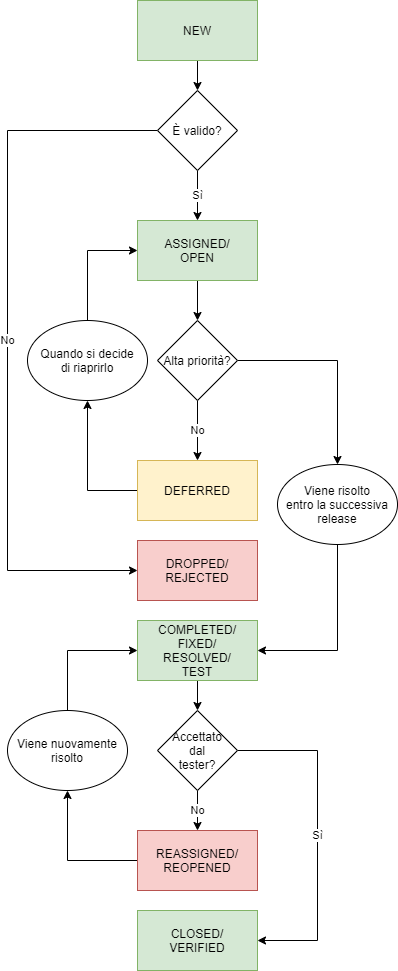
\includegraphics[scale=0.6]{img/003.png}
		\caption{Esempio di ciclo di vita del bug}
		\label{fig: 003}
	\end{center}
\end{figure}

\subsection{Status}
\begin{table}[]
\begin{tabular}{|l|l|}
\hline
\textbf{Status} & \textbf{Status alternativo} \\ \hline
NEW             &                             \\ \hline
ASSIGNED        & OPEN                        \\ \hline
DEFERRED        &                             \\ \hline
DROPPED         & REJECTED                    \\ \hline
COMPLETED       & FIXED, RESOLVED, TEST       \\ \hline
REASSIGNED      & REOPENED                    \\ \hline
CLOSED          & VERIFIED                    \\ \hline
\end{tabular}
\end{table}

\subsubsection{Spiegazione}
\paragraph{NEW}
Il tester ha trovato il difetto e lo posta con status NEW. Il difetto deve ancora essere controllato e approvato. Si può passare ad ASSIGNED, DROPPED, DEFERRED
\paragraph{ASSIGNED/OPEN}
Il test/development/progect leader studia il nuovo bug e se lo considera valido lo assegna ad un membro del team di sviluppo. Il suo computo è di renderlo COMPLETED
\paragraph{DEFERRED}
Se un bug NEW e ASSIGNED viene considerato non fondamentale e quindi da correggere in una futura release, allora il bug diventa DEFERRED fino al momento opportuno
\paragraph{DROPPED/REJECTED}
Il test/development/progect leader studia il nuovo bug e se non lo considera valido lo segna come DROPPED/REJECTED. Segna il cambiamento anche con le ragioni che l'hanno portato a rifiutarlo
\paragraph{COMPLETED/FIXED/RESOLVED/TEST}
Se lo sviluppatore correge il bug, questo ora deve essere testato dal team di testing. Può passare a CLOSED o REASSIGNED
\paragraph{Caso residuale}
Se uno sviluppatore non riesce a risolvere un bug, alcune organizzazioni potrebbero offrire i seguenti codici:
\begin{itemize}
	\item \textbf{Won't/Can't fis}: Lo sviluppatore non riesce a risolvere il bug
	\item \textbf{Can't reproduce}: Lo sviluppatore non riesce a riprodurre il bug
	\item \textbf{Need more information}: Lo sviluppatore richiede più informazioni al tester
\end{itemize}
\paragraph{REASSIGNED/REOPENED}
Se il tester trova che il bug non è stato corretto completamente o parzialmente  allora lo riassegna allo sviluppatore
\paragraph{CLOSED/VERIFIED}
Se il tester/test leader verifica che il bug è stato corretto e non ci sono più problemi, allora lo chiude.


\subsection{Linee guida}
\begin{itemize}
	\item Assicurati che l'intero team comprenda cosa significhi ogni status
	\item Documenta ogni step
	\item Assicurati che ogni individuo capisca le sue responsabilità riguardo i bug
	\item Assicurati che ci siano abbastanza dettagli in ogni cambio di status
	\item Se si usa un programma di bug tracking, tenerlo sempre aggiornato
\end{itemize}


\section{Defect report}
È molto simile al test plan, serve a identificare e descrivere un bug trovato da un tester.

\begin{table}[]
\begin{tabular}{|c|l|}
\hline
\textbf{ID}                                                               & ID del bug (solitamente è automatizzato)                                                                                                                                          \\ \hline
\textbf{Project}                                                          & Nome del progetto                                                                                                                                                                 \\ \hline
\textbf{Product}                                                          & Nome del prodotto                                                                                                                                                                 \\ \hline
\textbf{\begin{tabular}[c]{@{}c@{}}Release \\ version\end{tabular}}       & Release del prodotto                                                                                                                                                              \\ \hline
\textbf{Module}                                                           & Modulo specifico afflitto dal bug                                                                                                                                                 \\ \hline
\textbf{\begin{tabular}[c]{@{}c@{}}Detected build\\ version\end{tabular}} & Build specifica afflitta dal bug                                                                                                                                                  \\ \hline
\textbf{Summary}                                                          & \begin{tabular}[c]{@{}l@{}}Sommario del difetto. Deve essere\\ chiara e concisa\end{tabular}                                                                                      \\ \hline
\textbf{Descrizione}                                                      & \begin{tabular}[c]{@{}l@{}}Descrizione dettagliata del bug. \\ Descrive il più possibile senza ripetersi\\ e senza usare termini complessi.\\ Semplice ma esaustiva.\end{tabular} \\ \hline
\textbf{\begin{tabular}[c]{@{}c@{}}Steps to\\ replicate\end{tabular}}     & Passi per replicare il bug                                                                                                                                                        \\ \hline
\textbf{Actual result}                                                    & Risultato ottenuto                                                                                                                                                                \\ \hline
\textbf{Expected result}                                                  & Risultato atteso                                                                                                                                                                  \\ \hline
\textbf{Attachments}                                                      & Allegati eventuali (screenshot, log)                                                                                                                                              \\ \hline
\textbf{Remarks}                                                          & Ogni commento addizionale                                                                                                                                                         \\ \hline
\textbf{Defect severity}                                                  & Vedi pagina \pageref{par: Defect severity}                                                                                                                                   \\ \hline
\textbf{Defect priority}                                                  & Vedi pagina \pageref{par: Defect priority}                                                                                                                                   \\ \hline
\textbf{Reported by}                                                      & Chi l'ha identificato                                                                                                                                                             \\ \hline
\textbf{Assigned to}                                                      & Chi è incaricato di risolvere il bug                                                                                                                                              \\ \hline
\textbf{Status}                                                           & Vedi pagina \pageref{par: Defect lifecycle}                                                                                                                                  \\ \hline
\textbf{\begin{tabular}[c]{@{}c@{}}Fixed build\\ version\end{tabular}}    & \begin{tabular}[c]{@{}l@{}}Versione della build nella quale il bug\\ è stato corretto\end{tabular}                                                                                \\ \hline
\end{tabular}
\end{table}

\subsection{Riportare i bug in maniera efficace}
\begin{itemize}
	\item \textbf{Sii specifico}:
		\begin{itemize}
			\item Specifica l'azione esatta, non un geerico "seleziona il pulsante B" ma "clicca sul pulsante B" o "Metti il focus sul pulsante B e premi ENTER"
			\item Nel caso di più percorsi, specifica il percorso intrapreso per arrivare al bug
			\item Non usare pronomi vaghi, sii sempre specifico
		\end{itemize}
	\item \textbf{Sii dettagliato}: Offri più dettagli, non meno. In altre parole, non essere pigro
	\item \textbf{Sii oggettivo}: Non usare aggettivi per descrivere le cose, solo sostantivi. "Non è stato corretto" va bene, "l'hai corretto di merda" no\footnote{Per più motivi anche ma vabbè}
	\item \textbf{Riproduci il bug}: Non lanciarti subito a compilare il bug report, prima prova a riprodurlo più volte. Nel caso tu non ci riesca segnala il bug specificando che non sei riuscito a riprodurlo nuovamente
	\item \textbf{Controlla il report}: Non premere subito "invia", rileggilo. \textbf{Rimuovi gli errori di battitura}.
\end{itemize}


\chapter{Metriche di analisi per i bug}
\section{Age}
Può essere misurata in:
\begin{itemize}
	\item tempo
	\item fasi
\end{itemize}

\subsection{Age (tempo)}
\paragraph{Definizione}
È la differenza tra la data di quando il bug è identificato alla data corrente (se ancora aperto) o alla data di chiusura.

\paragraph{Spiegazione}
\begin{itemize}
	\item I bug sono confermati e assegnati
	\item I difetti DROPPED non sono contati
	\item L'età può essere calcolata in ore o giorni
	\item "FIXED" significa che il bug è stato corretto e chiuso dal tester
\end{itemize}

\paragraph{Formula}
Semplicemente
\begin{center}
	$Bug age = Data di chiusura (O data corrente) - Data di identificazione$
\end{center}

\subsection{Age (fasi)}
\paragraph{Definizione}
È la differenza tra fase nella quale è stata identificata e quella nella quale è stata introdotta.

\paragraph{Spiegazione}
\begin{itemize}
	\item "fase primaria" è quando il bug è stato introdotto
	\item "fase secondaria" è quando il bug è stato identificato
\end{itemize}

\paragraph{Formula}
Semplicemente
\begin{center}
	$Bug age = fase secondaria - fase primaria$
\end{center}

\section{Density}
\paragraph{Definizione}
È il numero di bug identificati in un software/componente durante un preciso periodo di sviluppo/operatività diviso per la grandezza del software.

\paragraph{Spiegazione}
I bug sono:
\begin{itemize}
	\item Confermati
	\item I difetti DROPPED non sono contati
\end{itemize}

Il periodo può essere uno dei seguenti:
\begin{itemize}
	\item un intervallo temporale specifico
	\item Per ogni fase del ciclo di vita del software
	\item Per l'intero ciclo di vita del software
\end{itemize}

La grandezza del software è definita tramite:
\begin{itemize}
	\item Punti funzione (FP)
	\item Linee di codice
\end{itemize}

\paragraph{Formula}
\begin{center}
	$Densità = \frac{Numero di difetti}{Grandezza}$
\end{center}

\section{Efficienza di individuazione dei bug}
\paragraph{Definizione}
La Defect Detection Efficiency (DDE) è il numero di bug identificati durante una fase che sono stati introdotti nella stessa fase diviso per il totale dei bug introdotti in quella fase.

\paragraph{Spiegazione}
\begin{itemize}
	\item \textbf{Bug}
		\begin{itemize}
			\item Confermati
			\item I difetti DROPPED non sono contati
		\end{itemize}
	\item \textbf{Fase}
		\begin{itemize}
			\item Può essere una qualsiasi fase dove i bug sono introdotti E identificati
		\end{itemize}
	\item \textbf{Introduzione}
		\begin{itemize}
			\item La fase nella quale il bug è stato introdotto viene identificata analizzando il bug
		\end{itemize}
\end{itemize}

\paragraph{Formula}
\begin{center}
	$DDE = \frac{Numero di bug introdotti E identificati nella stessa fase}{Numero totale di bug introdotti nella fase} * 100 \% $
\end{center}

Ovviamente 100\% è ciò che si desidera raggiungere.

\section{Costo della qualità}
\paragraph{Definizione}
Il Cost of Quality (COQ) è una misura che quantifica il costo del controllo o della conformità e il costo del fallimento del controllo o della non conformità.

È il costo totale delle attività di qualità e spesso è diviso tra costi di prevenzione, di identificazione, per problemi interni ed esterni.

\paragraph{Spiegazione}
\begin{itemize}
	\item Costo di conformità
		\begin{itemize}
			\item Costo di prevenzione: Il costo che deriva dall'effort di prevenire i difetti
			\item Costo di identificazione: Il costo che deriva dall'effort di identificare i difetti
		\end{itemize}
	\item Costo di non conformità
		\begin{itemize}
			\item Costo per fallimento interno: Il costo che deriva dall'identificare i difetti e l'effort nel risolverli
			\item Costo per fallimento esterno: Il costo che deriva dall'identificazione dei bug da parte degli utenti e l'effort nel risolverli
		\end{itemize}
\end{itemize}

\paragraph{Formula}
Abbiamo tre formule:
\begin{center}
	Costo di conformità\\=\\costo di prevenzione\\+\\costo di identificazione
	\rule{\textwidth}{0.4pt}
	Costo di non conformità\\=\\Costo per fallimento interno\\+\\Costo per fallimento esterno
	\rule{\textwidth}{0.4pt}
	Costo della qualità (COQ)\\=\\Costo di conformità\\+\\Costo di non conformità
\end{center}

\chapter{Junit - Corso udemy}
\href{https://www.udemy.com/course/junit-tutorial-for-beginners-with-java-examples/}{Corso Udemy - Learn Java Unit Testing with JUnit in 20 steps}.
\href{https://www.udemy.com/course/learn-unit-testing-with-spring-boot/}{Corso Udemy - Master Java Unit Testing with Spring Boot \& Mockito}.
In informatica JUnit è un framework di unit testing per il linguaggio di programmazione Java.

Siamo alla versione 5 (Jupiter). 

I file di test devono essere messi in una cartella separata chiamata test (per convenzione). In quella cartella emuleremo la struttura dei package della cartella src in modo da aggiungere significatività al posizionamento dei test, collegandoli intuitivamente alle classi che testano.

Ricordiamo prima di tutto le differenze tra unit test (pagina \pageref{par: unit test}) e integration test (pagina \pageref{par: integration test}).

Prima regola: il successo è la mancanza di fallimento. Questo perchè dobbiamo cercare i casi nei quali il test fallisce.

\section{Come si organizza un test?}
Si preparano i vari test annotandoli con @Test (vedremo poi le annotazioni). Al loro interno avremo le chiamate ai vari metodi (possibilmente un solo metodo per test) e per controllare i valori useremo gli assert. In un assert possiamo mettere che il risultato ottenuto dovrebbe essere uguale al risultato atteso. Nel caso differiscano avremo un fail.

Dobbiamo ricordarci che ci possiamo anche aspettare delle eccezioni derivanti dai metodi, bisogna considerarle. Un modo per gestirle in Junit 4 era @Test(Expected exception). In Junit 5 abbiamo assertThrows(Exception, metodo).

\subsection{Test per le eccezioni}
\begin{lstlisting}[language = Java]
// Vogliamo testare la funzione length per le stringhe
// Junit5
@Test
void testDiEsempio(){
	assertThrows(NullPointerException.class,
	
		() -> {
			null.length();
		}
		
	);
}

//Junit4
@Test(expected=NullPointerException.class)
void testDiEsempio(){
	null.length();
}

\end{lstlisting}

Questo è un esempio di programmazione funzionale, alla funzione viene passata l'eccezione e una lambda, ovvero viene passato il corpo della funzione da eseguire.

\subsection{Metodi public}
In JUnit 4 tutti i metodi di test dovevano essere public, in JUnit 5 non serve più

\subsection{Test parametrizzati in Junit 4}
\begin{lstlisting}[language = Java]
@RunWith(Parametrized.class)
public class testClass(){

	@Parameters
	public static Collection<String[]> testConditions(){
		String expectedOuputs[][] = {
			// Creazione collection
		}
		
		retrun Array.asList(expectedOutputs);
	}

	// Ora i metodi possono accedere direttamente
	// Alla collection come qualsiasi variabile
}
\end{lstlisting}


\subsection{Suite di test in Junit 4}
In Junit 5 si usa l'annotazione Tag.

Posso crearle tramite wizard, mi verranno anche proposte automaticamente le classi se voglio aggingerle. 
\begin{lstlisting}[language = Java]
@RunWith(Suite.class)
@SuiteClasses({array di classi})
public class tests(){
}
\end{lstlisting}

In questo modo si possono creare gruppi di test riguardanti funzioni specifiche
\subsection{@ValueSource}
\begin{lstlisting}[language = Java]
// Questo

@Test
void stringLengthControl(){
	assert("ABCD".length()>0);
	assert("ABC".length()>0);
	assert("AB".length()>0);
	assert("A".length()>0);
}

// e' uguale a

@ParametrizedTest
@ValueSource(string={"ABCD", "ABC", "AB", "A"})
void stringLengthControl(String str){
	assert(str.length()>0);
}
\end{lstlisting}

@ValueSource accetta in ingresso String[], int[], long[], double[]. Non serve scrivere il tipo di variabile all'interno della notazione perchè viene automaticamente riconosciuta.

\subsection{@CsvSource}

Se volessi controllare più valori alla volta dovrei sostituire @ValueSource con @CsvSource.
\begin{lstlisting}[language = Java]
@ParametrizedTest
@CsvSource(value={"ABCD, abcd", "ABC, abc", "AB, ab", "A, a"})
void capitalizedWordControl(String capitalStr, String str){
	assertEquals(capitalStr, str.toUpperCase());
}
\end{lstlisting}

Attenzione, prende solo Stringhe ma c'è un trucco. Infatti possiamo vedere nel seguente esempio che scrivendo un int come stringa questo venga automaticamente convertito perchè all'interno della firma del metodo è richiesto un int.
\begin{lstlisting}[language = Java]
@ParametrizedTest
@CsvSource(value={"ABCD, 4", "ABC, 3", "AB, 2", "A, 1"})
void capitalizedWordControl(String str, int length){
	assertEquals(str.length(), length);
}
\end{lstlisting}

\subsection{Timeout}
\begin{lstlisting}[language = Java]
// Junit 4
@Test(timeout = n)
public void performance(){
	// do something
}

//Junit 5
@Test
void performance(){
	assertTimeout(Duration.ofSeconds(n), () -> {
		//do something
	}
}

\end{lstlisting}

\section{Junit 4 vs Junit 5}
Junit 5 racchiude la Junit platform, Junit Jupiter e Junit vintage. L'ultima è ciò che permette di offrire supporto alle vecchie versioni.

In più sono state aggiunte alcune annotazione (confrontare tra le due sezioni) e alcuni attributi (expected e timeout) sono stati sostituiti da degli assert che prendono in ingresso delle lambda



\section{Tipi di assert Junit4}

\noindent\begin{table}[]
\small
\begin{tabular}{|l|l|}
\hline
\multicolumn{1}{|c|}{\textbf{Metodo}}                                                                                                                       & \multicolumn{1}{c|}{\textbf{Effetto}}                                                                                                                                                                      \\ \hline
\begin{tabular}[c]{@{}l@{}}assertArrayEquals(byte{[}{]} expecteds, \\ byte{[}{]} actuals)\end{tabular}                                                      & \begin{tabular}[c]{@{}l@{}}“Asserisce” che due array di byte\\ sono uguali\end{tabular}                                                                                                                    \\ \hline
\begin{tabular}[c]{@{}l@{}}assertArrayEquals(char{[}{]} expecteds, \\ char{[}{]} actuals)\end{tabular}                                                      & \begin{tabular}[c]{@{}l@{}}“Asserisce”\\ che due array di char sono uguali\end{tabular}                                                                                                                    \\ \hline
\begin{tabular}[c]{@{}l@{}}assertArrayEquals(int{[}{]} expecteds, \\ int{[}{]} actuals)\end{tabular}                                                        & “Asserisce” che due array di int sono uguali                                                                                                                                                               \\ \hline
\begin{tabular}[c]{@{}l@{}}assertArrayEquals(long{[}{]} expecteds, \\ long{[}{]} actuals)\end{tabular}                                                      & \begin{tabular}[c]{@{}l@{}}“Asserisce”\\ che due array di long sono uguali\end{tabular}                                                                                                                    \\ \hline
\begin{tabular}[c]{@{}l@{}}assertArrayEquals(java.lang.Object{[}{]} expecteds, \\ java.lang.Object{[}{]} actuals)\end{tabular}                              & \begin{tabular}[c]{@{}l@{}}“Asserisce” che due array di oggetti \\ sono uguali\end{tabular}                                                                                                                \\ \hline
\begin{tabular}[c]{@{}l@{}}assertArrayEquals(short{[}{]} expecteds, \\ short{[}{]} actuals)\end{tabular}                                                    & \begin{tabular}[c]{@{}l@{}}“Asserisce”\\ che due array di short sono uguali\end{tabular}                                                                                                                   \\ \hline
\begin{tabular}[c]{@{}l@{}}assertArrayEquals(java.lang.String message, \\ byte{[}{]} expecteds, \\ byte{[}{]} actuals)\end{tabular}                         & \begin{tabular}[c]{@{}l@{}}“Asserisce” che due array di byte \\ sono uguali. Nel caso non lo siano \\ viene mostrato message.\end{tabular}                                                                 \\ \hline
\begin{tabular}[c]{@{}l@{}}assertArrayEquals(java.lang.String message, \\ char{[}{]} expecteds, \\ char{[}{]} actuals)\end{tabular}                         & \begin{tabular}[c]{@{}l@{}}“Asserisce”\\ che due array di char sono uguali. \\ Nel caso non lo siano viene mostrato\\ message.\end{tabular}                                                                \\ \hline
\begin{tabular}[c]{@{}l@{}}assertArrayEquals(java.lang.String message, \\ int{[}{]} expecteds, \\ int{[}{]} actuals)\end{tabular}                           & \begin{tabular}[c]{@{}l@{}}“Asserisce” che due array di \\ int sono uguali. Nel caso\\ non lo siano viene mostrato message.\end{tabular}                                                                   \\ \hline
\begin{tabular}[c]{@{}l@{}}assertArrayEquals(java.lang.String message, \\ long{[}{]} expecteds, \\ long{[}{]} actuals)\end{tabular}                         & \begin{tabular}[c]{@{}l@{}}“Asserisce”\\ che due array di long sono uguali. \\ Nel caso non lo siano viene mostrato\\ message.\end{tabular}                                                                \\ \hline
\begin{tabular}[c]{@{}l@{}}assertArrayEquals(java.lang.String message, \\ java.lang.Object{[}{]} expecteds, \\ java.lang.Object{[}{]} actuals)\end{tabular} & \begin{tabular}[c]{@{}l@{}}“Asserisce” che due array di \\ oggetti sono uguali. Nel\\ caso non lo siano viene \\ mostrato message.\end{tabular}                                                            \\ \hline
\begin{tabular}[c]{@{}l@{}}assertArrayEquals(java.lang.String message, \\ short{[}{]} expecteds, \\ short{[}{]} actuals)\end{tabular}                       & \begin{tabular}[c]{@{}l@{}}“Asserisce”\\ che due array di short sono uguali. \\ Nel caso non lo siano viene mostrato\\ message\end{tabular}                                                                \\ \hline
\begin{tabular}[c]{@{}l@{}}assertEquals(double expected, \\ double actual)\end{tabular}                                                                     & \begin{tabular}[c]{@{}l@{}}Sconsigliato. \\ \\ Utilizzare invece\\ Il metodo\\ successivo.\end{tabular}                                                                                                    \\ \hline
\begin{tabular}[c]{@{}l@{}}assertEquals(double expected, \\ double actual, \\ double delta)\end{tabular}                                                    & \begin{tabular}[c]{@{}l@{}}“Asserisce”\\ che due double o float sono \\ uguali entro un certo delta.\end{tabular}                                                                                          \\ \hline
\begin{tabular}[c]{@{}l@{}}assertEquals(long expected, \\ long actual)\end{tabular}                                                                         & “Asserisce” che due long sono uguali.                                                                                                                                                                      \\ \hline
\end{tabular}
\end{table}

\noindent\begin{table}[]
\small
\begin{tabular}{|l|l|}
\hline
\multicolumn{1}{|c|}{\textbf{Metodo}}                                                                                                                       & \multicolumn{1}{c|}{\textbf{Effetto}}                                                                                                                                                                      \\ \hline
\begin{tabular}[c]{@{}l@{}}assertEquals(java.lang.Object{[}{]} expecteds, \\ java.lang.Object{[}{]} actuals)\end{tabular}                                   & \begin{tabular}[c]{@{}l@{}}Sconsigliato. \\ \\ Utilizzare invece\\ Il metodo assertArrayEquals.\end{tabular}                                                                                               \\ \hline
\begin{tabular}[c]{@{}l@{}}assertEquals(java.lang.Object expected, \\ java.lang.Object actual)\end{tabular}                                                 & \begin{tabular}[c]{@{}l@{}}“Asserisce” che due oggetti sono\\ uguali\end{tabular}                                                                                                                          \\ \hline
\begin{tabular}[c]{@{}l@{}}assertEquals(java.lang.String message, \\ double expected, \\ double actual)\end{tabular}                                        & \begin{tabular}[c]{@{}l@{}}Sconsigliato. \\ \\ Utilizzare invece\\ Il metodo successivo. Nel caso non lo siano\\ viene mostrato message.\end{tabular}                                                      \\ \hline
\begin{tabular}[c]{@{}l@{}}assertEquals(java.lang.String message, \\ double expected, \\ double actual, \\ double delta)\end{tabular}                       & \begin{tabular}[c]{@{}l@{}}“Asserisce” che due double o float \\ sono uguali entro un certo delta. \\ Nel caso non lo siano viene \\ mostrato message.\end{tabular}                                        \\ \hline
\begin{tabular}[c]{@{}l@{}}assertEquals(java.lang.String message, \\ long expected, \\ long actual)\end{tabular}                                            & \begin{tabular}[c]{@{}l@{}}“Asserisce” che due long sono uguali. \\ Nel caso non lo siano viene mostrato message.\end{tabular}                                                                             \\ \hline
\begin{tabular}[c]{@{}l@{}}assertEquals(java.lang.String message, \\ java.lang.Object{[}{]} expecteds, \\ java.lang.Object{[}{]} actuals)\end{tabular}      & \begin{tabular}[c]{@{}l@{}}Sconsigliato. \\ \\ Utilizzare invece\\ il metodo assertArrayEquals.\end{tabular}                                                                                               \\ \hline
\begin{tabular}[c]{@{}l@{}}assertEquals(java.lang.String message, \\ java.lang.Object expected, \\ java.lang.Object actual)\end{tabular}                    & \begin{tabular}[c]{@{}l@{}}“Asserisce” che due oggetti sono uguali. \\ Nel caso non lo siano viene mostrato message.\end{tabular}                                                                          
\\ \hline
\end{tabular}
\end{table}



\noindent\begin{table}[]
\small
\begin{tabular}{|l|l|}
\hline
\multicolumn{1}{|c|}{\textbf{Metodo}}                                                                                                                       & \multicolumn{1}{c|}{\textbf{Effetto}}                                                                                                                                                                      \\ \hline
assertFalse(boolean condition)                                                                                                                              & “Asserisce” che una condizione è falsa.                                                                                                                                                                    \\ \hline
\begin{tabular}[c]{@{}l@{}}assertFalse(java.lang.String message, \\ boolean condition)\end{tabular}                                                         & \begin{tabular}[c]{@{}l@{}}“Asserisce” che una condizione è \\falsa. \\ Nel caso non lo sia viene mostrato\\ message.\end{tabular}                                                                             \\ \hline
assertNotNull(java.lang.Object object)                                                                                                                      & “Asserisce” che un oggetto non è \\null.                                                                                                                                                                     \\ \hline
\begin{tabular}[c]{@{}l@{}}assertNotNull(java.lang.String message, \\ java.lang.Object object)\end{tabular}                                                 & \begin{tabular}[c]{@{}l@{}}“Asserisce” che un oggetto non è null. \\ Nel caso non lo sia viene mostrato \\message.\end{tabular}                                                                              \\ \hline
\begin{tabular}[c]{@{}l@{}}assertNotSame(java.lang.Object unexpected, \\ java.lang.Object actual)\end{tabular}                                              & \begin{tabular}[c]{@{}l@{}}“Asserisce” che due oggetti non sono \\ riferiti allo stesso indirizzo.\end{tabular}                                                                                            \\ \hline
\begin{tabular}[c]{@{}l@{}}assertNotSame(java.lang.String message, \\ java.lang.Object unexpected, \\ java.lang.Object actual)\end{tabular}                 & \begin{tabular}[c]{@{}l@{}}“Asserisce” che due oggetti non sono \\riferiti  allo stesso indirizzo. Nel caso \\ lo siano viene mostrato \\message.\end{tabular}                                                \\ \hline
assertNull(java.lang.Object object)                                                                                                                         & “Asserisce” che un oggetto è null.                                                                                                                                                                         \\ \hline
\begin{tabular}[c]{@{}l@{}}assertNull(java.lang.String message, \\ java.lang.Object object)\end{tabular}                                                    & \begin{tabular}[c]{@{}l@{}}“Asserisce” che un oggetto è null. \\ Nel caso lo sia viene mostrato message.\end{tabular}                                                                                      \\ \hline
\begin{tabular}[c]{@{}l@{}}assertSame(java.lang.Object expected,\\ java.lang.Object actual)\end{tabular}                                                    & \begin{tabular}[c]{@{}l@{}}“Asserisce” che due oggetti sono \\ riferiti allo stesso indirizzo.\end{tabular}                                                                                                \\ \hline
\begin{tabular}[c]{@{}l@{}}assertSame(java.lang.String message, \\ java.lang.Object expected, \\ java.lang.Object actual)\end{tabular}                      & \begin{tabular}[c]{@{}l@{}}“Asserisce” che due oggetti sono riferiti \\ allo stesso indirizzo. Nel caso non lo siano\\ viene mostrato message.\end{tabular}                                                \\ \hline
\begin{tabular}[c]{@{}l@{}}assertThat(java.lang.String reason, \\ T actual, \\ org.hamcrest.Matcher\textless{}T\textgreater matcher)\end{tabular}           & \begin{tabular}[c]{@{}l@{}}“Asserisce” che actual soddisfa la\\ condizione espressa in matcher. \\ Nel caso non lo sia viene \\ mostrato reason. \\ T è il tipo statico accettato da matcher.\end{tabular} \\ \hline
\begin{tabular}[c]{@{}l@{}}assertThat(T actual,\\ org.hamcrest.Matcher\textless{}T\textgreater matcher)\end{tabular}                                        & \begin{tabular}[c]{@{}l@{}}“Asserisce”   che actual soddisfa \\ la condizione espressa in matcher. \\ T è il tipo statico\\ accettato da matcher.\end{tabular}                                             \\ \hline
assertTrue(boolean condition)                                                                                                                               & \begin{tabular}[c]{@{}l@{}}“Asserisce” che una condizione \\ è vera.\end{tabular}                                                                                                                          \\ \hline
\begin{tabular}[c]{@{}l@{}}assertTrue(java.lang.String message, \\ boolean condition)\end{tabular}                                                          & \begin{tabular}[c]{@{}l@{}}“Asserisce” che una condizione \\ è vera. Nel caso non lo sia \\ viene mostrato message.\end{tabular}                                                                           \\ \hline
fail()                                                                                                                                                      & Fallisce un test senza messaggio.                                                                                                                                                                          \\ \hline
fail(java.lang.String message)                                                                                                                              & Fallisce un test con messaggio.                                                                                                                                                                            \\ \hline
assertThrows(java.lang.Exception exception, lambda)                                                                                                                              & Fallisce se il metodo non invoca\\ l'eccezione preventivata \\ \hline
\end{tabular}
\end{table}\footnote{"It's not much but it's honest work"

\textit{- Me about this table layout}}

\section{Assunzioni e teorie}
Le assunzioni sono test di verità per i test. Nel caso un'assunzione fallisca il test non fallisce, semplicemente non viene eseguito perchè non rientra nel caso di analisi.

Mentre un test coglie uno specifico caso, una teoria invece è un test più generico che può essere usato in un'infinità di casi. Vengono collegate alle assunzioni perchè, per discriminare i vari casi in modo da non creare un fallimento automatico la maggior parte delle volte, si creano delle assunzioni all'interno delle teorie. Ad esempio

\begin{lstlisting}[language = Java]
@RunWith(Theories.class)
public class UserTest {
    @DataPoint
    public static String GOOD_USERNAME = "optimus";
    @DataPoint
    public static String USERNAME_WITH_SLASH = "optimus/prime";

    @Theory
    public void filenameIncludesUsername(String username) {
        assumeThat(username, not(containsString("/")));
        assertThat(new User(username).configFileName(), containsString(username));
    }
}
\end{lstlisting}

Questo test rende chiaro che uno username dovrebbe essere incluso nel file di configurazione solo se non contiene uno slash. Un altro test o teoria potrebbe prendere il caso residuale.

\section{Regole}
Le regole permettono di modificare il comportamento di un test durante la sua esecuzione.

\subsection{TemporaryFolder}
TemporaryFolder permette la creazione di file e cartelle che sono cancellate quando il metodo termina. Nessuna eccezione è lanciata se la risorsa non può essere cancellata.

\begin{lstlisting}[language = Java]
public static class HasTempFolder {
  @Rule
  public final TemporaryFolder folder = new TemporaryFolder();

  @Test
  public void testUsingTempFolder() throws IOException {
    File createdFile = folder.newFile("myfile.txt");
    File createdFolder = folder.newFolder("subfolder");
    // ...
  }
} 
\end{lstlisting}

\subsection{ExternalResource}
È una classe base per la costruzione di regole che crea una risorsa esterna prima di un test (file, socket, server, connessione al database, ecc.) e garantisce di chiuderla dopo il test.

\begin{lstlisting}[language = Java]
public static class UsesExternalResource {
  Server myServer = new Server();
  
  @Rule
  public final ExternalResource resource = new ExternalResource() {
    @Override
    protected void before() throws Throwable {
      myServer.connect();
    };
    
    @Override
    protected void after() {
      myServer.disconnect();
    };
  };
  
  @Test
  public void testFoo() {
    new Client().run(myServer);
  }
}
\end{lstlisting}

\subsection{ErrorCollector}
Permette di continuare l'esecuzione di un test anche dopo che il primo problema viene identificato (per esempio per raccogliere tutti gli errori e fare un report unico).

\begin{lstlisting}[language = Java]
public static class UsesErrorCollectorTwice {
  @Rule
  public final ErrorCollector collector = new ErrorCollector();
  
  @Test
  public void example() {
    collector.addError(new Throwable("first thing went wrong"));
    collector.addError(new Throwable("second thing went wrong"));
  }
}
\end{lstlisting}

\subsection{Verifier}
È una classe base per altre regole, permette di rendere un test positivo un test negativo se una verifica fallisce.
\begin{lstlisting}[language = Java]
public static class UsesVerifier {
  
  private static String sequence;
  
  @Rule
  public final Verifier collector = new Verifier() {
    @Override
    protected void verify() {
      sequence += "verify ";
    }
  };

  @Test
  public void example() {
    sequence += "test ";
  }
  
  @Test
  public void verifierRunsAfterTest() {
    sequence = "";
    assertThat(testResult(UsesVerifier.class), isSuccessful());
    assertEquals("test verify ", sequence);
  }

}
\end{lstlisting}

\subsection{TestWatcher}
È fondamentalmente un Logger per i test.

\subsection{TestName}
Permette di utilizzare il nome del test all'interno dei metodi.

\begin{lstlisting}[language = Java]
public class NameRuleTest {
  @Rule
  public final TestName name = new TestName();
  
  @Test
  public void testA() {
    assertEquals("testA", name.getMethodName());
  }
  
  @Test
  public void testB() {
    assertEquals("testB", name.getMethodName());
  }
}
\end{lstlisting}

\subsection{Timeout}
Applica lo stesso timeout a tutti i test
\begin{lstlisting}[language = Java]
public static class HasGlobalTimeout {
  public static String log;
  
  @Rule
  public final TestRule globalTimeout = Timeout.millis(20);
  
  @Test
  public void testInfiniteLoop1() {
    log += "ran1";
    for(;;) {}
  }
  
  @Test
  public void testInfiniteLoop2() {
    log += "ran2";
    for(;;) {}
  }
}
\end{lstlisting}

\subsection{ExpectedException}
Permette di specificare il tipo di eccezione atteso e il messaggio.

\begin{lstlisting}[language = Java]
public static class HasExpectedException {
  @Rule
  public final ExpectedException thrown = ExpectedException.none();

  @Test
  public void throwsNothing() {

  }

  @Test
  public void throwsNullPointerException() {
    thrown.expect(NullPointerException.class);
    throw new NullPointerException();
  }

  @Test
  public void throwsNullPointerExceptionWithMessage() {
    thrown.expect(NullPointerException.class);
    thrown.expectMessage("happened?");
    thrown.expectMessage(startsWith("What"));
    throw new NullPointerException("What happened?");
  }
}
\end{lstlisting}

\subsection{ClassRule}
Semplicemente estende il concetto di regola per il test ad una regola per tutta la classe. Tutti i runner parent e anche le altre classi della suite della regola.

\begin{lstlisting}[language = Java]
@RunWith(Suite.class)
@SuiteClasses({A.class, B.class, C.class})
public class UsesExternalResource {
  public static final Server myServer = new Server();

  @ClassRule
  public static final ExternalResource resource = new ExternalResource() {
    @Override
    protected void before() throws Throwable {
      myServer.connect();
    };

    @Override
    protected void after() {
      myServer.disconnect();
    };
  };
}
\end{lstlisting}

\subsection{RuleChain}
Permette di ordinare le regole.
\begin{lstlisting}[language = Java]
public static class UseRuleChain {
    @Rule
    public final TestRule chain = RuleChain
                           .outerRule(new LoggingRule("outer rule"))
                           .around(new LoggingRule("middle rule"))
                           .around(new LoggingRule("inner rule"));

    @Test
    public void example() {
        assertTrue(true);
    }
}
\end{lstlisting}

\subsection{Regole personalizzate}
Si possono creare delle regole o estendendo la classe ExternalResource oppure implementando l'interfaccia TestRule.
\begin{lstlisting}[language = Java]
public class TestLogger implements TestRule {
  private Logger logger;

  public Logger getLogger() {
    return this.logger;
  }

  @Override
  public Statement apply(final Statement base, final Description description) {
    return new Statement() {
      @Override
      public void evaluate() throws Throwable {
        logger = Logger.getLogger(description.getTestClass().getName() + '.' + description.getDisplayName());
        base.evaluate();
      }
    };
  }
}

//  E la sua applicazione
public class MyLoggerTest {

  @Rule
  public final TestLogger logger = new TestLogger();

  @Test
  public void checkOutMyLogger() {
    final Logger log = logger.getLogger();
    log.warn("Your test is showing!");
  }

}
\end{lstlisting}

\section{Categorie}
Le categorie permettono di eseguire solo i metodi che hanno l'annotazione @IncludeCategory o i sottotipi di quella categoria. Si possono usare classi o interfacce per quest'inclusione.

\begin{lstlisting}[language = Java]
public interface FastTests { /* category marker */ }
public interface SlowTests { /* category marker */ }

public class A {
  @Test
  public void a() {
    fail();
  }

  @Category(SlowTests.class)
  @Test
  public void b() {
  }
}

@Category({SlowTests.class, FastTests.class})
public class B {
  @Test
  public void c() {

  }
}

@RunWith(Categories.class)
@IncludeCategory(SlowTests.class)
@SuiteClasses( { A.class, B.class }) // Note that Categories is a kind of Suite
public class SlowTestSuite {
  // Will run A.b and B.c, but not A.a
}

@RunWith(Categories.class)
@IncludeCategory(SlowTests.class)
@ExcludeCategory(FastTests.class)
@SuiteClasses( { A.class, B.class }) // Note that Categories is a kind of Suite
public class SlowTestSuite {
  // Will run A.b, but not A.a or B.c
}
\end{lstlisting}

\section{Multithreade}
Per testare un codice alla ricerca di problemi di concorrenza si passano una Collection di Runnable che possono essere usati per controllare errori di multithreading.

\begin{lstlisting}[language = Java]
public static void assertConcurrent(final String message, final List<? extends Runnable> runnables, final int maxTimeoutSeconds) throws InterruptedException {
    final int numThreads = runnables.size();
    final List<Throwable> exceptions = Collections.synchronizedList(new ArrayList<Throwable>());
    final ExecutorService threadPool = Executors.newFixedThreadPool(numThreads);
    try {
        final CountDownLatch allExecutorThreadsReady = new CountDownLatch(numThreads);
        final CountDownLatch afterInitBlocker = new CountDownLatch(1);
        final CountDownLatch allDone = new CountDownLatch(numThreads);
        for (final Runnable submittedTestRunnable : runnables) {
            threadPool.submit(new Runnable() {
                public void run() {
                    allExecutorThreadsReady.countDown();
                    try {
                        afterInitBlocker.await();
                        submittedTestRunnable.run();
                    } catch (final Throwable e) {
                        exceptions.add(e);
                    } finally {
                        allDone.countDown();
                    }
                }
            });
        }
        // wait until all threads are ready
        assertTrue("Timeout initializing threads! Perform long lasting initializations before passing runnables to assertConcurrent", allExecutorThreadsReady.await(runnables.size() * 10, TimeUnit.MILLISECONDS));
        // start all test runners
        afterInitBlocker.countDown();
        assertTrue(message +" timeout! More than" + maxTimeoutSeconds + "seconds", allDone.await(maxTimeoutSeconds, TimeUnit.SECONDS));
    } finally {
        threadPool.shutdownNow();
    }
    assertTrue(message + "failed with exception(s)" + exceptions, exceptions.isEmpty());
}
\end{lstlisting}

\section{Annotazioni Junit 4}
\begin{itemize}
	\item \textbf{@Test}: segna che il successivo metodo è un test e il suo risultato sarà gestito da JUnit
	\item \textbf{@Test(expected = exception.class}: segna che il successivo metodo è un test e dovrebbe lanciare l'eccezione attesa
	\item \textbf{@Test(timeout = n)}: Per impostare un limite massimo temporale nell'esecuzione a n secondi
	\item \textbf{@BeforeAll}: Viene eseguito come prima cosa
	\item \textbf{@Before}: Viene eseguito come prima di ogni test
	\item \textbf{@AfterAll}: Viene eseguito dopo tutti i test
	\item \textbf{@After}: Viene eseguito dopo ogni test
	\item \textbf{@DisplayName(stringa)}: Personalizza il nome del test mostrato nei risultati JUnit
	\item \textbf{@Ignores}: Permette di disabilitare alcuni test
	\item \textbf{@Category(class)}: serve per riunire assieme un gruppo di test
	\item \textbf{@RunWith(class)}: a livello di classe segnala che tipo di test verrà eseguito
\end{itemize}

\section{Annotazioni Junit5}
\begin{itemize}
	\item \textbf{@Test}: segna che il successivo metodo è un test e il suo risultato sarà gestito da JUnit
	\item \textbf{@BeforeClass}: Viene eseguito come prima cosa
	\item \textbf{@BeforeEach}: Viene eseguito prima di ogni test
		\begin{itemize}
			\item[] Nell'intestazione del metodo si può mettere come variabile passata (TestInfo [nome variabile) per segnare quale test sta per essere eseguito
		\end{itemize}
	\item \textbf{@AfterClass}: Viene eseguito dopo tutti i test
	\item \textbf{@AfterEach}: Viene eseguito dopo ogni test
		\begin{itemize}
			\item[] Nell'intestazione del metodo si può mettere come variabile passata (TestInfo [nome variabile) per segnare quale test è stato eseguito
		\end{itemize}
	\item \textbf{@DisplayName(stringa)}: Personalizza il nome del test mostrato nei risultati JUnit
	\item \textbf{@ValueSource(creazione variabile)}: Permette di passare più variabili per creare un test parametrizzato
	\item \textbf{@ParametrizedTest(name = String}: Per segnare che questo test prende in input i dati da un'annotazione @ValueSource. Nella stringa possiamo scrivere cosa comparirà nel riassunto di Junit e possiamo anche accedere ai campi del Value/CsvSource tramite {n} come notazione per la posizione all'interno della tupla.
	\item \textbf{@CsvSource(value={insieme di tuple})}: Nel caso debba dare più variabili in ingresso per il test
	\item \textbf{@RepeatedTest(int)}: Ripete il test n volte
	\item \textbf{@Disabled}: Permette di disabilitare alcuni test
	\item \textbf{@Tag}: A livello di classe o metodo, permette di filtrare i test.
	\item \textbf{@Nested}: Ci permette di inserire una classe di test dentro ad un'altra. È comodo per rendere più leggibili le suite di test all'interno del riassunto.
\end{itemize}

\chapter{Mockito - corso Udemy}
\href{https://www.udemy.com/course/learn-unit-testing-with-spring-boot/}{Corso Udemy - Master Java Unit Testing with Spring Boot \& Mockito}.


\section{Stub}
Il creare Mock è essenziale per creare degli unit test. Questo perchè il mocking ci permette di "fingere" che ci sia un servizio dove richiesto, senza dover effettivamente accedere alle risorse, inizializzarle, accedere al database, ecc. Semplicemente diamo una classe finta con ciò che ci serve per il test.

Per farlo dobbiamo creare quindi delle finte implementazioni delle classi. Un modo è farlo hardcoded, ovvero scriverle direttamente. Non molto corretto nè manutenibile.

L'altra è usare Mockito.
\begin{center}
	\begin{lstlisting}[language = Java]
Classe service = mock(Classe.class);
	\end{lstlisting}
\end{center}

Abbiamo così una finta classe. Ma per aggiungervi dati?
Esistono i metodi when.then. \pageref{par: whenthen}

È utile usare l'annotazione @Before o @BeforeClass per creare gli stub prima di tutto.

\section{@InjectMocks e @Mock}
Perchè però dover fare un inject del mock come se fosse una classe normale quando Mockito ci aiuta anche in quello?

Semplicemente con tre annotazioni possiamo creare un mock in maniera pulita.

\begin{lstlisting}[language = Java]
@RunWith(MockitoJUnitRunner.class)
public class someClassTest(){
	
	// Questa e' la classe che testiamo
	@InjectMocks
	SomeClass class;
	
	@Mock
	SomeAuxiliaryClass	auxClass;
	
	...
}
\end{lstlisting}


Facendo così segniamo che nella classe SomeClass ci saranno delle classi interne che avranno bisogno di Mock.

Segnando queste classi con Mock vengono automaticamente istanziate come mock.

\section{when-then}\label{par: whenthen}
per personalizzare cosa accade durante le chiamate.
Ad esempio:
\begin{lstlisting}[language = Java]
when(service.retrieveAll()).thenReturn(new int[]{1, 2, 3});
\end{lstlisting}

Semplicemente ora la chiamata offrirà direttamente questo array.

E se volessi diversi risultati diverse volte? Posso concatenare più thenReturn che verranno eseguiti in ordine, quindi, ad esempio:
\begin{lstlisting}[language = Java]
when(mock.size()).thenReturn(5).thenReturn(10);
assertEquals(mock.size(), 5);
assertEquals(mock.size(), 10);
\end{lstlisting}

In questo caso il test avrà successo.

\section{Any}
Mockito offre un argument matcher, ovvero dei metodi chiamati anyInt, antString, ecc. che sono semplicemente dei placeholder per qualsiasi valore venga passato loro.

\section{Verify(mock)}
Permette di verificare che certi metodi vengano chiamati con certi valori.
Ad esempio:
\begin{lstlisting}[language = Java]
verify(mock, times(2)).get(anyInt());
\end{lstlisting}

Controlla che venga chiamato con qualsiasi indice due volte. Ci sono anche altri metodi statici che controllano quante volte venga chiamato un metodo.
\begin{itemize}
	\item never()
	\item atLeast(times)
	\item times(times)
	\item atMost(times)
	\item atLeastOnce()
\end{itemize}

\section{Argument capture}
L'argument capture serve a intercettare i valori risultanti dalle chiamate per poi essere salvati all'interno del captor. Non è semplicissimo, procediamo ad esempi:
\begin{lstlisting}[language = Java]
class MockitoArgumentCaptorExamples {

	@Test
	void test() {
		// Creiamo il mock della classe		
		MathUtils mockMathUtils = mock(MathUtils.class);
		
		// Sostituiamo due chiamate per il mock
		when(mockMathUtils.add(1, 1))
			.thenReturn(2);
		when(mockMathUtils.isInteger(anyString()))
			.thenReturn(true);

		// Creiamo due ArgumentCaptor nella vecchia
		// maniera
		ArgumentCaptor acInteger = 
			ArgumentCaptor.forClass(Integer.class);
		ArgumentCaptor acString = 
			ArgumentCaptor.forClass(String.class);
	
		
		assertEquals(2, mockMathUtils.add(1, 1));
		assertTrue(mockMathUtils.isInteger("1"));
		assertTrue(mockMathUtils.isInteger("999"));

		/* Verify mi permette di controllare le chiamate
		* effettuate ad un preciso metodo.
		* Inserendo captor.capure() al posto
		* dell'argomento che dovrebbe verificare
		* permettiamo al captor di intercettarlo
		* e di salvarlo all'interno della sua
		* collection
		*/
		verify(mockMathUtils)
			.add(acInteger.capture(), acInteger.capture());
		
		/* Salviamo in una lista tutti i valori
		* intercettati. Se avessimo un solo valore
		* ci basterebbe fare getValue()
		*/
		List allValues = acInteger.getAllValues();
		assertEquals(List.of(1, 1), allValues);
	
		/* Come prima effettuiamo la verifica
		* al metodo chiamato all'interno di
		* assertTrue. Chiamandolo con un 
		* ArgumentCaptor per le stringhe
		* abbiamo una conversione implicita
		*/
		verify(mockMathUtils, times(2))
			.isInteger(acString.capture());
			
			
		List allStringValues = acString.getAllValues();
		assertEquals(List.of("1", "999"), allStringValues);
	}


	/* Definisco l'argument Captor
	* Questa notazione e' uguale a
	* ArgumentCaptor acLong = ArgumentCaptor.forClass(Long.class);
	* La particolarita' e' che non serve piu'
	* definire la classe che dovra' catturare
	*/
	@Captor ArgumentCaptor acLong;
	
	@Test
	void test() {
		MathUtils mockMathUtils = mock(MathUtils.class);
		
		when(mockMathUtils.squareLong(2L))
			.thenReturn(4L);
			
		assertEquals(4L, mockMathUtils.squareLong(2L));
		
		/* Notiamo che anche senza aver definito la classe
		* intercettata, comunque l'ArgumentCaptor riesce
		* a intercettare correttamente il dato
		*/
		verify(mockMathUtils).squareLong(acLong.capture());
		
		assertTrue(2 == acLong.getValue());
	}
}
\end{lstlisting}

\section{@Spy}
Il problema principale dei mock è che non mantengono il comportamento della classe originale. Quindi anche aggiungendo dati al suo interno la chiamata a size, ad esempio, rimarrebbe sempre 0.

Come fare quindi ad emulare il comportamento statefull della classe originale?

\begin{lstlisting}[language = Java]
@Test
public void whenNotUseSpyAnnotation_thenCorrect() {
    List<String> spyList = 
    	Mockito.spy(new ArrayList<String>());
     
    spyList.add("one");
    spyList.add("two");
 
    Mockito.verify(spyList).add("one");
    Mockito.verify(spyList).add("two");
 
    assertEquals(2, spyList.size());
 
    Mockito.doReturn(100).when(spyList).size();
    assertEquals(100, spyList.size());
}

@Spy
List<String> spiedList = new ArrayList<String>();
 
@Test
public void whenUseSpyAnnotation_thenSpyIsInjectedCorrectly() {
    spiedList.add("one");
    spiedList.add("two");
 
    Mockito.verify(spiedList).add("one");
    Mockito.verify(spiedList).add("two");
 
    assertEquals(2, spiedList.size());
 
    Mockito.doReturn(100).when(spiedList).size();
    assertEquals(100, spiedList.size());
\end{lstlisting}

Come possiamo vedere l'inizializzazione della classe mock tramite spy ci permette di mantenere lo stesso comportamento della classe originale. Quindi, quando ci troviamo a modificare i dati usiamo i metodi \textbf{reali} del mock mentre quando usiamo i metodi sono semplicemente stub.

Le classi spy vengono create per controllare cosa accade nella classe originale.

\section{Eccezioni}
Si possono lanciare eccezioni tramite mockito.
\begin{lstlisting}[language = Java]
doThrow(new RuntimeException()).when(mockedList).clear();

//following throws RuntimeException:
mockedList.clear();
\end{lstlisting}

\section{Ordine delle verifiche}
In certi casi si può voler controllare l'ordine delle chiamate, per questo viene in aiuto inOrder.
\begin{lstlisting}[language = Java]
// A. Single mock whose methods must be invoked in a particular order
List singleMock = mock(List.class);

//using a single mock
singleMock.add("was added first");
singleMock.add("was added second");

//create an inOrder verifier for a single mock
InOrder inOrder = inOrder(singleMock);

//following will make sure that add is first called with "was added first", then with "was added second"
inOrder.verify(singleMock).add("was added first");
inOrder.verify(singleMock).add("was added second");

// B. Multiple mocks that must be used in a particular order
List firstMock = mock(List.class);
List secondMock = mock(List.class);

//using mocks
firstMock.add("was called first");
secondMock.add("was called second");

//create inOrder object passing any mocks that need to be verified in order
InOrder inOrder = inOrder(firstMock, secondMock);

//following will make sure that firstMock was called before secondMock
inOrder.verify(firstMock).add("was called first");
inOrder.verify(secondMock).add("was called second");

// Oh, and A + B can be mixed together at will
\end{lstlisting}
La verifica è flessibile, non dobbiamo verificare tutte le chiamate, solo quelle che ci interessano.

Quando si crea un oggetto InOrder si possono anche passare i mock che ci interessano per al verifica.

\section{Verifica delle interazioni}
Per capire se ci sono interazioni tra chiamate si può usare si possono verificare le interazioni.
\begin{lstlisting}[language = Java]
//using mocks - only mockOne is interacted
mockOne.add("one");

//ordinary verification
verify(mockOne).add("one");

//verify that method was never called on a mock
verify(mockOne, never()).add("two");

//verify that other mocks were not interacted
verifyZeroInteractions(mockTwo, mockThree);
\end{lstlisting}

\section{Chiamate consecutive}
Magari vogliamo che in base alla chiamata un metodo di un mock restituisca un output differente. Per questo si possono concatenare i vari return.
\begin{lstlisting}[language = Java]
when(mock.someMethod("some arg"))
  .thenThrow(new RuntimeException())
  .thenReturn("foo");

//First call: throws runtime exception:
mock.someMethod("some arg");

//Second call: prints "foo"
System.out.println(mock.someMethod("some arg"));

//Any consecutive call: prints "foo" as well (last stubbing wins).
System.out.println(mock.someMethod("some arg"));

// Versione breve
when(mock.someMethod("some arg"))
   .thenReturn("one", "two", "three");
\end{lstlisting}

Attenzione! se volessimo usare più return in realtà il secondo sovrascriverebbe il primo.
\begin{lstlisting}[language = Java]
//All mock.someMethod("some arg") calls will return "two"
when(mock.someMethod("some arg"))
  .thenReturn("one")
when(mock.someMethod("some arg"))
  .thenReturn("two")
\end{lstlisting}

\section{Metodi aggiuntivi}
Quando si deve rispondere ad una chiamata when si possono usare altri metodi rispetto ai soliti. Sono essenziali quando si vuole:
\begin{itemize}
	\item Creare uno stub dei metodi void
	\item Creare uno stub sugli oggetti spy
	\item Creare uno stub di un metodo più di una volta per cambiare il comportamento di un mock durante il test
\end{itemize}

\begin{itemize}
	\item \textbf{doReturn(Object)}
	\item \textbf{doThrow(Throwable...)}
	\item \textbf{doThrow(Class)}
	\item \textbf{doAnswer(Answer)}
	\item \textbf{doNothing()}
	\item \textbf{doCallRealMethod()}
\end{itemize}

\section{Reset dei mock}
Generalmente non viene usato perchè è un sintomo di un test scritto male. Sarebbe meglio creare un nuovo mock.




\section{Limiti di Mockito 2}
\begin{itemize}
	\item Non può emulare i metodi statici
	\item Non può emulare i costruttori
	\item Non può emulare equals() e hashCode()
	\item Non si può usare mock() in un thenReturn()
	\item Non si possono emulare i metodi final
\end{itemize}

Per emulare i metodi privati, statici e i costruttori (non è una buona pratica) si può usare \href{https://github.com/powermock/powermock}{powermock}, un altro framework di testing.

\chapter{Unit and integration testing con Spring boot e mockito}
\section{Unit testing sui controller}
Una semplice annotazione, @WebMvcTest(controller.class), ci permette di emulare il comportamento del controller all'interno del test.

In più ci serve anche annotare la classe con @RunWith(SpringRunner.class) per segnalare che la classe va eseguita tramite Spring.

Quando eseguiamo una classe con @WebMvcTest abbiamo già un bean collegato, MockMvc, che ci permette di invocare la funzione perform() per sequire le HTTP request. Un po' di confusione, vediamo il codice.
\begin{lstlisting}[language = Java]
// Controller
@RestController
public class controllerBase{
	
	@GetMapping("/hello-world")
	public String helloWorld(){
		return "Hello world!";
	}
	
	/* Il controller convertira' automaticamente
	* l'item in un JSON che conterra'
	* tutti i dati dell'item
	*/
	@GetMapping("/dummy-item")
	public Item dummyItem(){
		// id, name, price, quantity
		return new Item(1, "ball", 10, 100);
	}
}

// Test
@RunWith(SpringRunner.class)
@WebMvcTest(controllerBase.class)
public class controllerBaseTest{

	@Autowired
	private MockMvc mockMvc;
	
	// Test per Hello World
	@Test
	public void helloWorldTest(){
	
		/* Creiamo la HTTP request */
		RequestBuilder request = MockMvcRequestBuilders
			.get("/hello-world")
			.accept(MediaType.APPLICATION_JSON);
		
		/* Prendiamo il result
		* eseguiamo la richiesta
		* ci aspettiamo che restituisca uno status 200
		* ci aspettiamo che contenga una stringa
		* salviamo il risultato
		*/
		MvcResult result = mockMvc
			.perform(request)
			.andExpect(status().is(OK)) // Status 200
			.andExpect(content.string("Hello world"))
			.andReturn();
		
		assertEquals("Hello World", result
			.getResponse
			.getContentAsString());
	}
	
	@Test
	public void dummyItemTest(){
		/* Creiamo la HTTP request */
		RequestBuilder request = MockMvcRequestBuilders
			.get("/dummy-item")
			.accept(MediaType.APPLICATION_JSON);
			
		/* abbiamo cambiato il tipo da String a json
		* questo perche' string si aspetta una corrispondenza
		* perfetta tra cio' che viene chiesto e 
		* cio' che viene restituito.
		* json ci permette di trattarlo invece come
		* un json, chiedendo anche solo alcuni dati
		* e non tutti e senza aver paura che 
		* alcuni spazi siano sbagliati
		*/
		MvcResult result = mockMvc
			.perform(request)
			.andExpect(status().is(OK)) // Status 200
			.andExpect(content
				.json("{id: 1, name:Ball, price:10"));
			.andReturn()

	}
}
\end{lstlisting}

\section{JsonAssert}
Framework a parte per controllare i JSON.

\begin{lstlisting}[language = Java]
JSONAssert.assertEquals(expected, actual, strict);
\end{lstlisting}
I primi due spiegano bene cosa vogliano, il terzo invece prescrive la modalità di controllo.
\begin{itemize}
	\item true: vuole tutti i campi della risposta
	\item false: può anche essere un sottoinsieme
\end{itemize}

Notare che gli spazi non vengono considerati e l'unico caso di carattere di escape utile è quando abbiamo uno spazio all'interno dei dati.



\chapter*{Link utili}
\begin{itemize}
	\item[] \href{http://xunitpatterns.com/}{xunitpatterns.com}, libro disponibile gratuitamente online per studiare svariati pattern di testing
	\item[] \href{https://junit.org/junit4/}{Documentazione Junit 4}
	\item[] \href{https://junit.org/junit5/}{Documentazione Junit 5}
	\item[] \href{https://site.mockito.org/}{Mockito}
	\item[] \href{https://github.com/powermock/powermock}{powermock}
	\item[] \href{https://joel-costigliola.github.io/assertj/}{AssertJ}
	
\end{itemize}

\end{document}
